% \documentclass[aip,apl]{revtex4-1}
% \documentclass[aps,prl,preprint,groupedaddress]{revtex4-1}
\documentclass[aps,prb,twocolumn,superscriptaddress,reprint]{revtex4-1}
\usepackage{graphicx}
\usepackage[utf8]{inputenc}
% \usepackage[pdfusetitle]{hyperref}
\usepackage{amsmath}
\usepackage{siunitx}
\usepackage{xcolor, color}
\usepackage{float}
\usepackage{multirow}
\usepackage[version=3]{mhchem} % Formula subscripts using \ce{}
\usepackage{latexsym,epsfig,amssymb,,subcaption,pictex,amsfonts}
\usepackage{tocloft}
\usepackage{setspace}
\usepackage{siunitx}

\graphicspath{{figures/}}
\newcommand{\re}[1]{\textcolor{red}{#1}}

\newcommand\T{\rule{0pt}{2.6ex}}       % Top strut
\newcommand\B{\rule[-1.2ex]{0pt}{0pt}} % Bottom strut
\newcommand*\mycommand[1]{\texttt{\emph{#1}}}
\newcommand{\etal}{{\it et al.}\ }

\begin{document}

\title[NMC]{LiNi\textsubscript{x}Mn\textsubscript{y}Co\textsubscript{z}O\textsubscript{2} (NMC) Cathodes for Li-ion Batteries: from Atoms to Devices}

\author{Mazharul M. Islam}
\affiliation{Department of Chemistry, University of Bath, Claverton Down, Bath BA2 7AY, UK}
\affiliation{The Faraday Institution, Quad One, Becquerel Avenue, Harwell Campus, Didcot, OX11 0RA, UK}

\author{Lucy M. Morgan}
\affiliation{Department of Chemistry, University of Bath, Claverton Down, Bath BA2 7AY, UK}
\affiliation{The Faraday Institution, Quad One, Becquerel Avenue, Harwell Campus, Didcot, OX11 0RA, UK}

\author{Hui Yang}
\affiliation{Department of Materials, Imperial College London, London SW7 2AZ, UK}
\affiliation{The Faraday Institution, Quad One, Becquerel Avenue, Harwell Campus, Didcot, OX11 0RA, UK}

\author{Abir Ghosh}
\affiliation{Department of Mechanical Engineering, Imperial College London, London, SW7 2AZ, UK}
\affiliation{The Faraday Institution, Quad One, Becquerel Avenue, Harwell Campus, Didcot, OX11 0RA, UK}

\author{Anisha N. Patel}
\affiliation{Department of Mechanical Engineering, Imperial College London, London, SW7 2AZ, UK}
\affiliation{The Faraday Institution, Quad One, Becquerel Avenue, Harwell Campus, Didcot, OX11 0RA, UK}

\author{Kieran O'Regan}
\affiliation{School of Metallurgy and Materials, University of Birmingham, Edgbaston, Birmingham, BT15 2TT, UK}
\affiliation{The Faraday Institution, Quad One, Becquerel Avenue, Harwell Campus, Didcot, OX11 0RA, UK}

\author{Emma Kendrick}
\affiliation{School of Metallurgy and Materials, University of Birmingham, Edgbaston, Birmingham, BT15 2TT, UK}
\affiliation{The Faraday Institution, Quad One, Becquerel Avenue, Harwell Campus, Didcot, OX11 0RA, UK}

\author{Monica Marinescu}
\affiliation{Department of Mechanical Engineering, Imperial College London, London, SW7 2AZ, UK}
\affiliation{The Faraday Institution, Quad One, Becquerel Avenue, Harwell Campus, Didcot, OX11 0RA, UK}

\author{Gregory Offer}
\affiliation{Department of Mechanical Engineering, Imperial College London, London, SW7 2AZ, UK}
\affiliation{The Faraday Institution, Quad One, Becquerel Avenue, Harwell Campus, Didcot, OX11 0RA, UK}

\author{Benjamin J. Morgan}
\affiliation{Department of Chemistry, University of Bath, Claverton Down, Bath BA2 7AY, UK}
\affiliation{The Faraday Institution, Quad One, Becquerel Avenue, Harwell Campus, Didcot, OX11 0RA, UK}

\author{Saiful M. Islam}
\affiliation{Department of Chemistry, University of Bath, Claverton Down, Bath BA2 7AY, UK}
\affiliation{The Faraday Institution, Quad One, Becquerel Avenue, Harwell Campus, Didcot, OX11 0RA, UK}

\author{Jacqueline Edge}
\affiliation{Department of Mechanical Engineering, Imperial College London, London, SW7 2AZ, UK}
\affiliation{The Faraday Institution, Quad One, Becquerel Avenue, Harwell Campus, Didcot, OX11 0RA, UK}
\email{j.edge@imperial.ac.uk}

\author{Aron Walsh}
\affiliation{Department of Materials, Imperial College London, London SW7 2AZ, UK}
\affiliation{Department of Materials Science and Engineering, Yonsei University, Seoul 03722, Korea}
\affiliation{The Faraday Institution, Quad One, Becquerel Avenue, Harwell Campus, Didcot, OX11 0RA, UK}
\email{a.walsh@imperial.ac.uk}

\date{\today}

\begin{abstract}
The first generation of cathodes in commercial lithium-ion batteries are based on layered transition metal oxides. Research on ternary compounds such as LiCoO$_2$ evolved into mixed-metal systems, notably Li(Ni,Mn,Co)O$_2$ (NMC), which allows significant tuning of the physical properties. Despite its widespread application, the fundamental understanding of NMC is limited. Here, we review the latest insights from multi-scale modelling, bridging between the redox phenomena that occur at an atomistic level to the transport of ions and electrons across an operating device. We discuss changes in the electronic and vibrational structure through the NMC compositional space and how these link to continuum models of electrochemical charge/discharge cycling. Finally, we outline the remaining challenges for predictive models of high-performance batteries including capturing the relevant device bottlenecks and chemical degradation processes such as oxygen evolution.
\end{abstract}


\maketitle

\section{Introduction}
Rechargeable lithium ion batteries (LIBs) are currently the most promising power source for a wide range of technologies ranging from portable consumer electronics, automotive vehicles, and mobility equipment, to large scale renewable grid energy storage applications \cite{}.  However, for such applications, further advancements in LIBs are essential in order to achieve higher energy densities, longer charge-discharge life cycles, lower costs, and higher stabilities to meet the requirements of these technologies.  Current LIB systems are complicated by a variety of physico-chemical processes that take place within dynamic microstructures of the battery material (anode and cathode), during cell cycling. 
Extensive research efforts are underway to improve existing battery materials, developing a better understanding of the degradation mechanisms in LIBs. This review summaries multi-scale models and experimental techniques essential for understanding and optimizing battery performance.

Layered lithium transition metal oxides (e.g. Li$M$O$_{2}$, where $M$ = Co, Ni, Mn, etc.) are considered as the first generation cathode materials in commercial LIBs, which although possessing a theoretical specific capacity of 270 mAh/g show a limited practical capacity below 200 mAh/g \cite{Myung2017}. LiCoO$_{2}$ is problematic due to high cost of cobalt and the ethical questions regarding the geopolitical issues \cite{mo_impact_2018}. Other oxides such as Li$_{x}$NiO$_{2}$ show capacity fade and poor safety \cite{min_comparative_2016}, while Li$_{x}$Mn$_{2}$O$_{4}$ shows low capacity \cite{tian_performance_2018} as cathode materials.

A promising alternative is to partially replace Co in LiCoO$_{2}$ with Ni and Mn to obtain layered LiNi$_{x}$Mn$_{y}$Co$_{z}$O$_{2}$ ($x+y+z=1$) system, commonly abbreviated as NMC \cite{rozier_review_2015}. These systems show improved electrochemical performance while reducing the material cost \cite{ohzuku_layered_2001}. The composition of Ni, Mn, and Co can be tuned to obtain various NMC structures. For the application in long-range electric vehicles companies are now switching to LiNi$_{0.8}$Mn$_{0.1}$Co$_{0.1}$O$_{2}$ (NMC811) for the commercial production [ref1]\cite{}, as use of nickel-rich cathodes increases energy density, while reducing cobalt content. Ni-rich NMCs are considered to be the cathode of choice for future all-solid-state LIBs \cite{Myung2017}. In the range of studies showcased here, we have employed combined multi-scale modelling and experimental approaches, focusing on the Ni-rich NMC811 system to investigate the structure and properties relationship of NMC cathodes.

We have investigated the influence of the valence states of transition metals (TMs) on the stability and structure-property relationships of NMC811 using various first principles electronic structure methods. \re{[Rana-Paper]\cite{rana}} Four strategies were employed to quantify the oxidation states of the transition metals: comparison of magnetic moments, analysis of Wannier functions, calculation of projected density of states (PDOS), and analysis of the Jahn-Teller distortion effect.\cite{yang2019highly,yang2020chemical} Based on this data, the lowest energy structures comprised 1Ni$^{2+}$, 7Ni$^{3+}$, 1Mn$^{4+}$, and 1Co$^{3+}$ in the transition metal layer. A disproportionation from 2Ni$^{3+}$ to Ni$^{2+}$ + Ni$^{4+}$ is also evident in the pristine NMC811 structure. These findings are important for the improvement of electrochemical behaviour of cathodes as well as for the understanding of structural degradation of LIBs during cycling.

On the dynamic properties, phonon dispersion, phonon density of states, and thermal properties have been reported for Li$M$O ($M$ = Co, Ni, Mn) and various NMC compositions. The oxidation and spin states of the transition metal cations are found to strongly influence the structural dynamics.  The low phonon frequency phonon branches that are mainly contributed by the TM elements move toward a higher-frequency regime with increasing Ni content. This indicates the strengthening of the TM-O bonds in the Ni-rich compounds, which is consistent with the general decreasing lattice constant in the c-axis \cite{sun_electronic_2017}. The thermal conductivity of NMC is suppressed with decreasing Co content and increasing Ni/Mn content. NMC811 was predicted to have a thermal conductivity of 10.3 Wm$^{-1}$K$^{-1}$ (see \ref{figure})and $\sim$4 times lower than that of LiCoO$_{2}$ \cite{yang2019highly,yang2020chemical}. Additionally, NMC811 has the challenges of having low structural stability, thermal stability, and elastic modulus.

Li-ion migration during charge/discharge processes is an important phenomenon that governs the battery operation. For this reason we have employed first principles DFT and Classical Molecular Dynamics (MD) approaches to study the local Li hop mechanisms and long-range Li diffusion mechanisms. Our continuous work untangles the complex structural and electrochemical influence on forming classical MD interatomic potentials and the considerations required to conduct Li diffusion studies at different states of charge. This work has led to the creation of a new potential fitting code and a wide discussion on whether the complex NMC structure is possible to represent using a classical model \cite{Morgan2020}.

The lifetime of the NMC811 cathode material is limited due to faster capacity fading, impedance rise, and loss of active material. These occur due to various degradation mechanisms such as mechanical degradation, passivation layer formation, oxygen evolution, transition metal dissolution, and growth of the cathode solid electrolyte interphase (CSEI) \cite{Li2019degra}. In a study showcased here [Abir-Paper] \cite{}, continuum models have been developed to understand these degradation phenomena and to solve these issues by informing material design. Concurrently the thermodynamic and kinetic behaviour of NMC811 have been studied using the Doyle-Fuller-Newman (DFN) model \cite{hui2020param} to optimize the performance of LIBs. The advantage of continuum-scale models is they bridge atomistic level understandings with the experimental observations at the cell level during cycling and calendar ageing. In this regard, the modelling data will be further complemented with experimental measurements on various degradative processes affecting NMC811 application in LIBs, including the above-mentioned degradation mechanisms.

\section{DFT Calculation of Vibrational Structure (Hui)}
Traditional crystallography presents the image of atoms being held in static positions through stiff chemical bonds, while atoms are vibrating within crystals, which is the natural interpretation of temperature. Lattice dynamics has since been introduced in order to gain a more complete picture of crystalline materials. Lattice dynamics of a crystal has since been widely used in vibrational spectra and thermal transport.

Although still an emerging area of interest, there are several studies reporting on the dynamic properties of NMC. Recently, \citeauthor{yang2020chemical} reported the harmonic phonon dispersion for the \ce{LiMO2} (M = Ni, Co, Mn) endpoints in the NMC oxide system. \cite{yang2020chemical} Their results revel that the Jahn-Teller (JT) effect is more pronounced in the crystalline \ce{LiMnO2} with three distinct bond lengths for the TM-O bonds. They found that the medium and low frequency modes are mainly due to motion of Li and TMs, while the high frequency modes ($>$ 14 THz) are vibrations involving the TM and O atoms. The phonons also provide information of a group theoretic analysis within the group assigns the irreducible representations of the acoustic and optic branches. Of these, some modes are infra-red (IR) active or Raman active, which is comparable with experimental IR/Raman spectra, with differences likely due to the volume expansion at finite temperature. \cite{yang2019highly} For NMC alloy systems, \citeauthor{sun_electronic_2017} showed that longitude acoustic frequency increases in the phonon dispersion curves from NMC333 to NMC811 (Figure \ref{figure_phonon}) due to the weaker electron screening effect.\cite{sun_electronic_2017}

\begin{figure}[h]
  \centering
    \resizebox{8cm}{!}{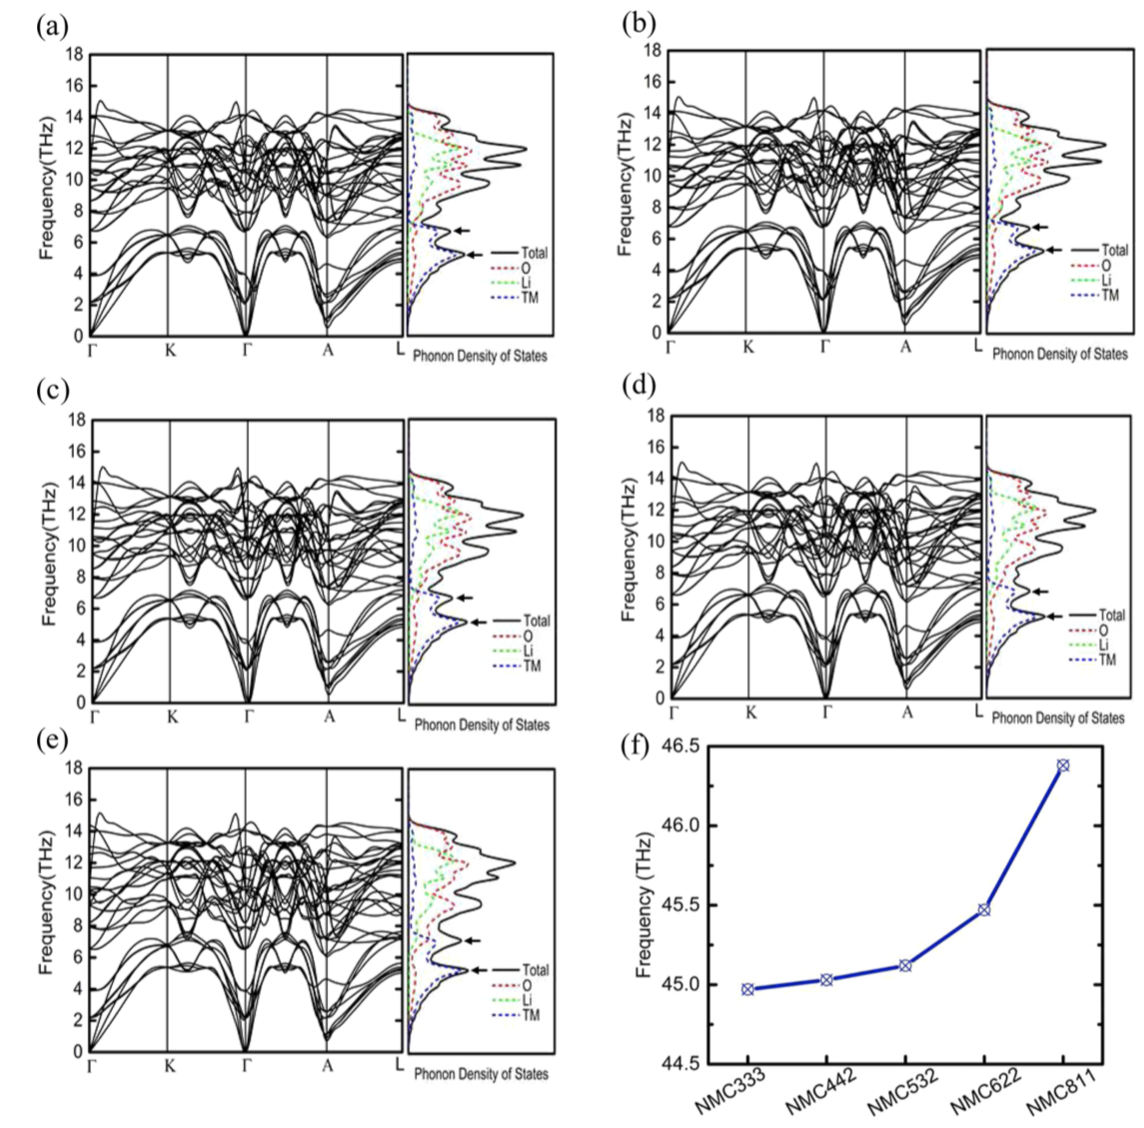
\includegraphics{Figures/P_phonon.png}}
    \caption{(a-e)Phonon dispersion and phonon density of states of NMC333, NMC442, NMC532, NMC622, and NMC811, respectively. DOS curves are showed on the right panel. (f) Longitude acoustic frequency in the five NMC compounds around the Gamma point, from Ref. \citenum{sun_electronic_2017}.}
  \label{figure_phonon}
\end{figure}

The electrochemical and thermal properties of Li(Ni$_x$Mn$_y$Co$_z$)O$_2$ are strongly dependent on its composition. An increase of the Ni content results in an increase in specific discharge capacity and total residual lithium content, however, the corresponding capacity retention and safety characteristics gradually decreased, Figure \ref{figure_thermal}. \cite{noh2013comparison} 

\begin{figure}[h]
  \centering
    \resizebox{7cm}{!}{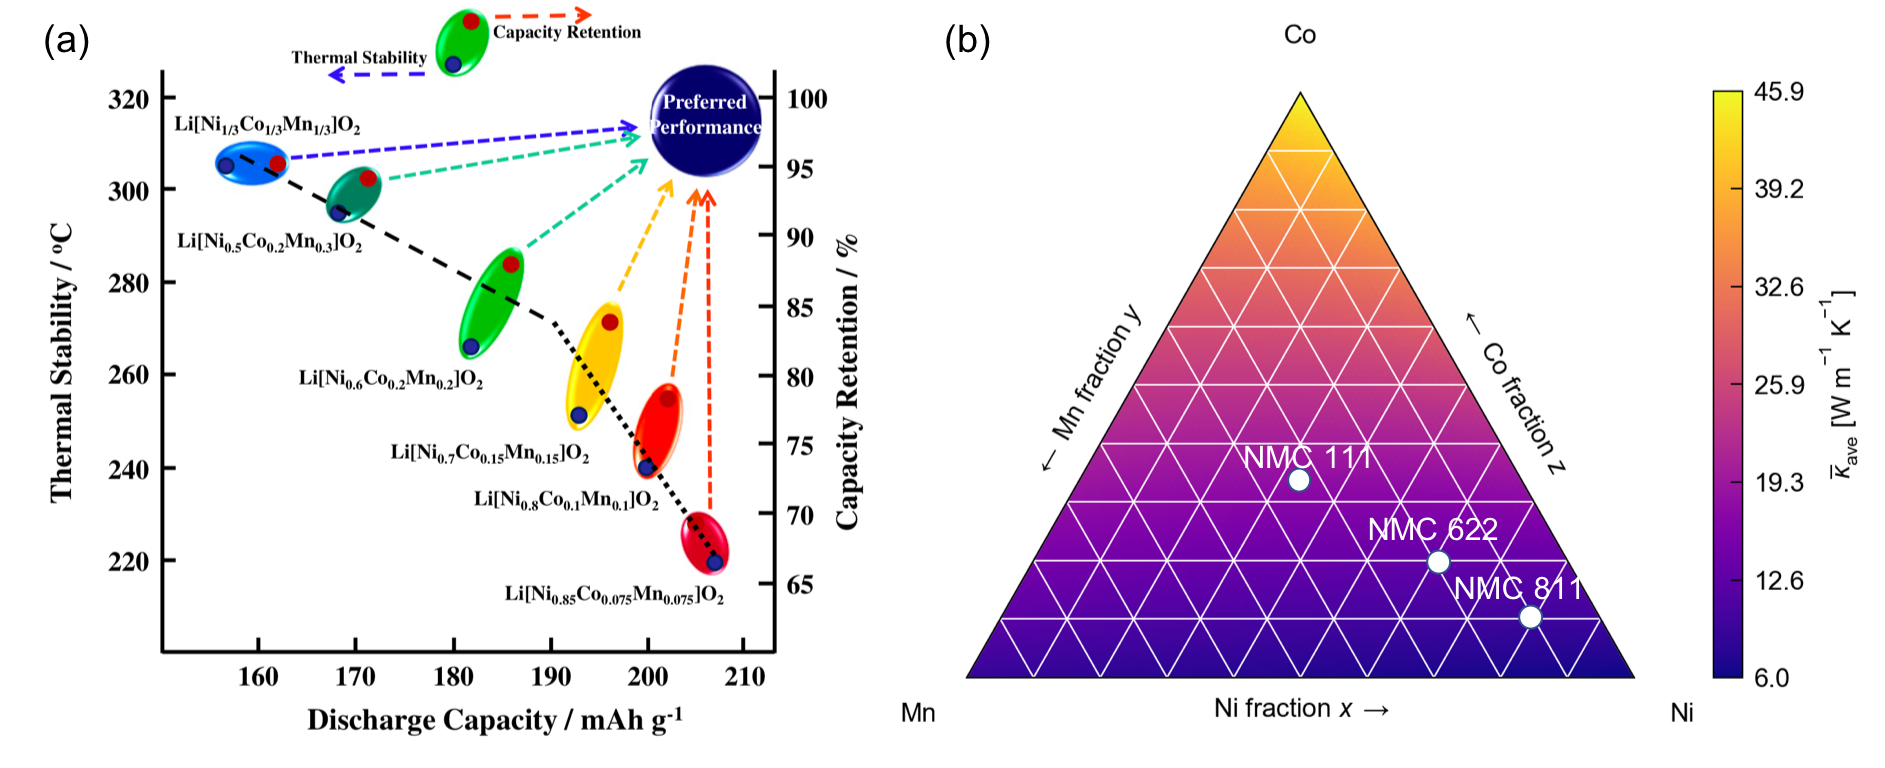
\includegraphics{Figures/P_thermal.png}}
    \caption{Relation between discharge capacity, and thermal stability and capacity retention of Li/Li(Ni$_x$Mn$_y$Co$_z$)O$_2$ (x = 0.33, 0.5, 0.6, 0.7, 0.8 and 0.85), from Ref. \citenum{noh2013comparison}.}
  \label{figure_thermal}
\end{figure}

Theoretical studies also report that increasing Ni/Mn content in NMC leads to lattice thermal conductivity suppression.\cite{yang2020chemical} Thermal conductivity decays exponentially with increasing temperature due to enhanced phonon scattering resulting from the larger thermal population of phonon modes. Figure \ref{figure_kappa} shows that at room temperature NMC811 has the lowest predicted thermal conductivity of 9.3 \SI{}{W.m^{-1}.K^{-1}} , while NMC622 and NMC111 are higher at 13.3 and 17.9 \SI{}{W.m^{-1}.K^{-1}}, respectively. In most devices, the thermal conductivity is much lower than these theoretical upper limit.\cite{takahata2002thermal,chen2006thermal} Both having smaller grain sizes  in poly-crystalline cathode materials and charging (delithiation) softens the lattice leading to smaller phonon velocities and stronger phonon scattering. \cite{feng2020quantum,xia2020high} These studies show the accessibility of tuning cathode material properties systematically by optimizing the ratio of the transition metals in NMC alloys, and further lower the barriers for battery cathode design.

\begin{figure}[]
  \centering
    \resizebox{8cm}{!}{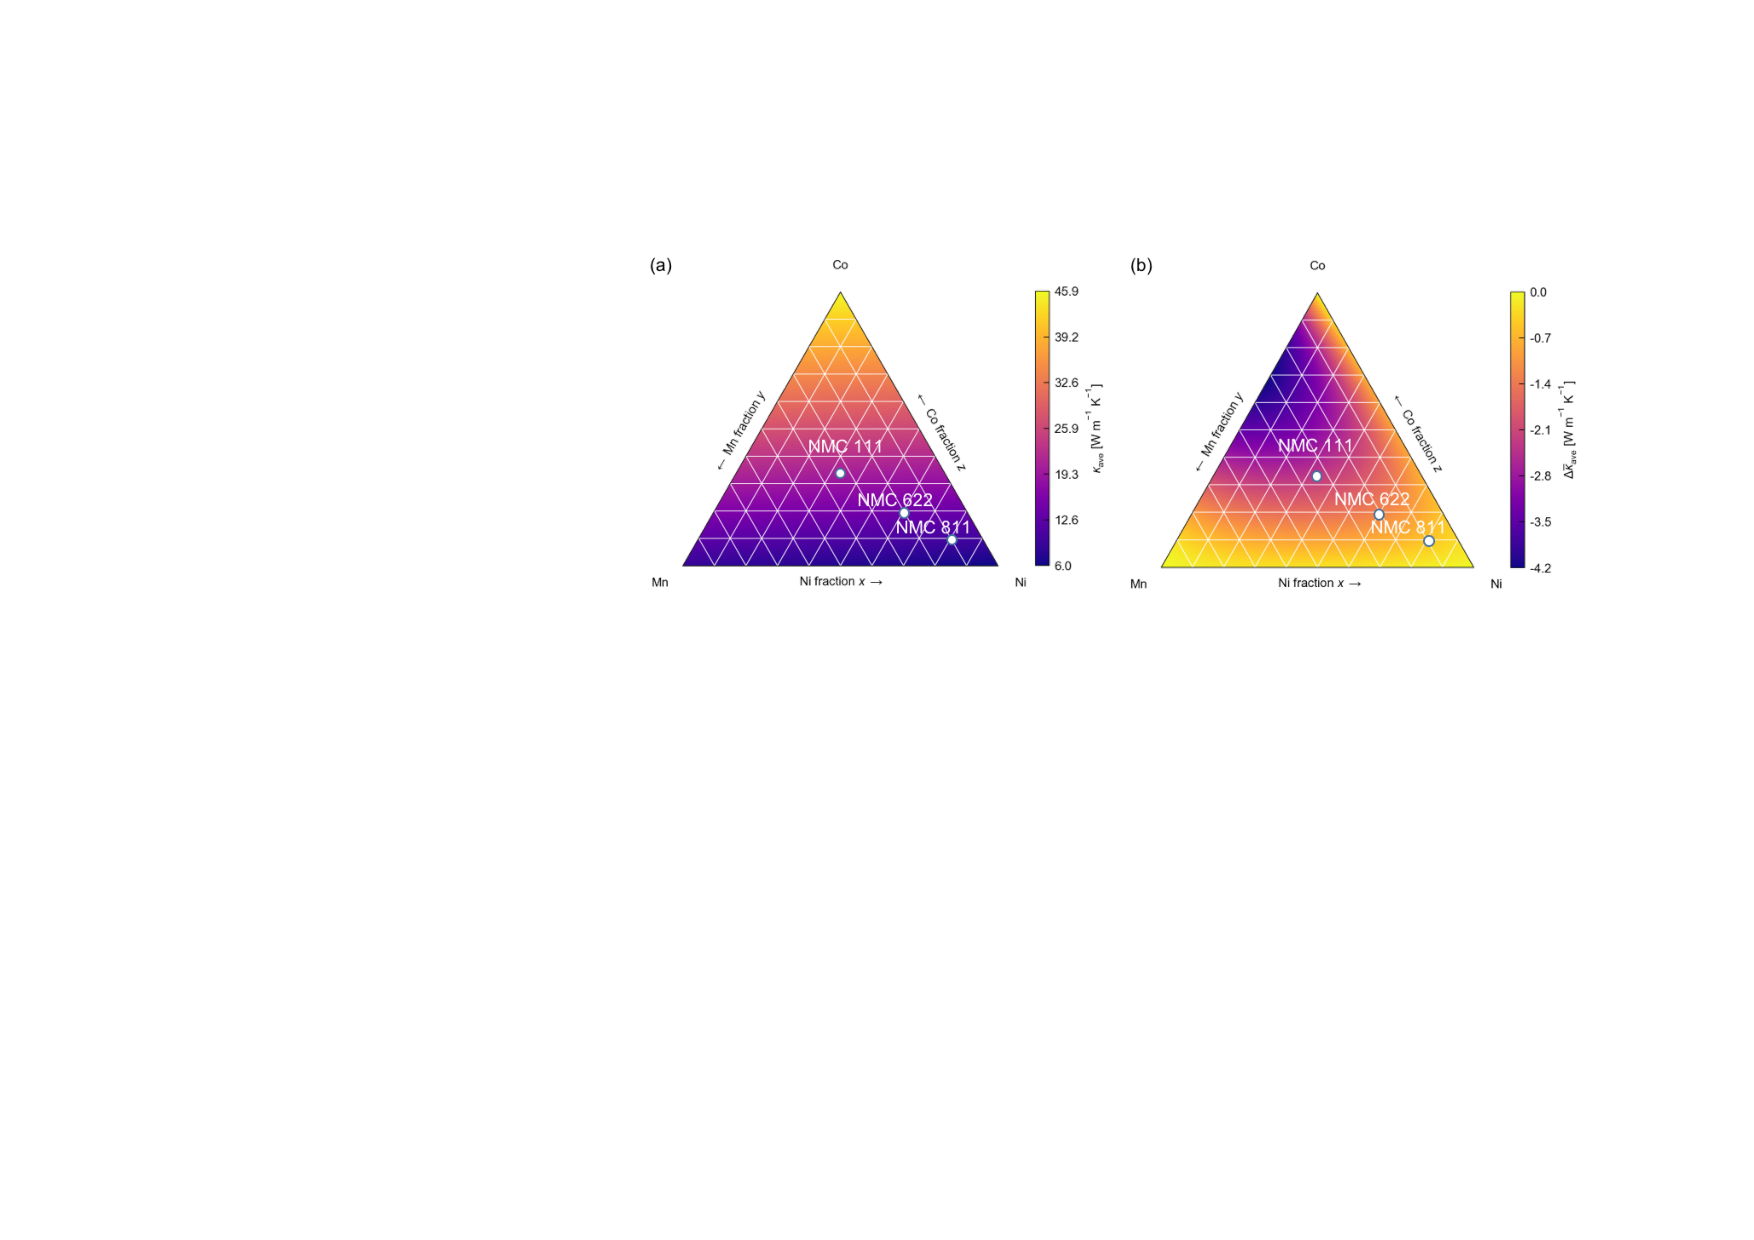
\includegraphics{Figures/P1.pdf}}
    \caption{Ternary map of the thermal conductivity map $\kappa$ of the NMC system. (a) is generated assuming a physical mixture of the pure components , while (b) shows the change in $\kappa$ if proportional mixing at the transition metal site induces changes in the average mass and mass variation at the cation site, from Ref. \citenum{yang2020chemical}. }
  \label{figure_kappa}
\end{figure}

\section{DFT Elucidation of Structure and Properties Relationship (Rana)}
The practical use of NMC materials in LIBs faces various challenges including structural degradation and capacity fading. One of the major issues is the spin interaction of transition metal (TM) ions. \cite{Feng-2019, Xia2018} Different compositions and charge distributions of the transition metals result in the appearance of various valence states, e.g. Ni$^{2+}$, Ni$^{3+}$, Ni$^{4+}$, Co$^{3+}$, Co$^{4+}$, Mn$^{4+}$. \cite{Xiao_NanoEner2018} The coexistence and interactions of these multivalent TM spins make it difficult to construct a unique ground state for NMCs. \cite{Xiao_NanoEner2018} Understanding the range of transition metal oxidation states, and the roles they play in degradation processes, is therefore crucial for the improvement of these promising cathode materials.

Due to the complex ordering and multivalent nature of transition metals, it is difficult to determine their precise oxidation states as well as the valence changes occured during electrochemical cycling.  Ni is the key redox active element in NMC. Experimentally, nickel in NMC811 remains as mixed Ni$^{2+}$ and Ni$^{3+}$ oxidation states, with the average value close to 3+. \cite{Zhu_JMatChemA2019,Katharina-chemmater,Kondrakov_JPhysChemC2017} For the fully lithiated system, Ni$^{4+}$ is not present, and would only be present upon lithium extraction. \cite{Katharina-chemmater} However, Ni disproportionation in pristine NMC811 has not been reported experimentally. In a previous computational study \cite{HChen_PhysRevB2011},  Ni disproportionation, $2$Ni$^{3+}\rightarrow$Ni$^{2+} + $Ni$^{4+}$, has been discussed for LiNiO$_2$. Charge disproportionation is observed in other cathode materials such as in pristine LiMn$_2$O$_4$ where  $2$Mn$^{3+}\rightarrow$Mn$^{2+} + $Mn$^{4+}$ disproprtionation is considered to be the main responsible for Mn dissolution which in turn leads to the capacity fading and anode poisoning. \cite{Parmar-LMO-2020,PASQUALINI2017} %in computational studies on layered transition metal oxides, for example LiNiO$_2$.\cite{HChen_PhysRevB2011} 

Previous theoretical investigations have studied the influence of transition metal oxidation states on NMC materials, \cite{Dan-Thomas-chemmater,Sun_JPhysChemC2017,Dixit_JPhysChemC2017,Dixit_JPhysChemC2017,Hoang_ACSChemMater2016,Dixit_JElecSoc2017} where the presence of  Ni$^{2}$, Ni$^{3+}$ and Ni$^{4+}$ is reported in NMC811. These studies, employing the DFT+\textit{U} approach, reported a gradual closing of the band gap from NMC111 to NMC811 indicating the metallic character of Ni-rich compounds. This was in contrast to typical properties of the Li$M$O$_{2}$ structures which show semiconducting properties with clear band gaps. \cite{Sun_JPhysChemC2017,Dixit_JPhysChemC2017, Hoang_ACSChemMater2016,Dixit_JElecSoc2017} DFT calculations employing the HSE06 hybrid functional predict the band gap of NMC111 to be \SI{2.88}{eV} \cite{Hoang_ACSChemMater2016}, whereas that with DFT+\textit{U} is less than \SI{0.3}{eV}.\cite{Sun_JPhysChemC2017} This illustrates that the previous studies using DFT+\textit{U} do not reproduce the electronic structure for NMC811 correctly. Another important aspect is that these studies have employed Jahn-Teller distortion and atomic magnetic moments, which have difficulties assigning oxidation states of mixed TMs unambiguously.

Recently, \re{\citeauthor{rana}} have employed HF-DFT hybrid HSE06 functional coupled with Wannier function analysis to assign oxidation states in Ni rich NMC811 (LiNi$_{0.8}$Mn$_{0.1}$Co$_{0.1}$O$_{2}$). \cite{rana} The effect of transition metal ordering and oxidation state configuration on the relative stability of different NMC811 models was studied. The limitations of other approaches to assign oxidation states, such as analysis of magnetic moments and Jahn-Teller distortions, were also illustrated.

By randomly varying the atomic positions of Ni, Mn and Co in the lattice, \re{\citeauthor{rana}} created 53 structural models of NMC811. The total energy values of these structures were calculated by full optimization of the fractional coordinates and the lattice parameters. The calculated energies depend on the transition metal arrangement, resulting in preferred TM configurations. This finding is in contrast to recent suggestions that the transition metal cations in NMC811 are randomly distributed. \cite{Sun_JPhysChemC2017} The stability of the NMC811 varies due to the distribution and interaction of mixed oxidation states of the TM ions (Ni$^{2+}$/Ni$^{3+}$/Ni$^{4+}$, Co$^{3+}$, and Mn$^{4+}$). This is in line with the experimental observations that the spin interactions of TM ions influence the ground state stability of NMC. \cite{Xiao_NanoEner2018}  Figure \ref{fig:stability}(a) presents the proportion of Ni ions in a given oxidation state for all considered models obtained with the HSE06 functional, ordered by relative energies per formula unit. \cite{rana} The distribution of transition metals is the only difference between these 53 NMC811 models. Therefore, it is clear that the relative energies of NMC811 structures depends strongly on how the mixed oxidation state transition metals are ordered and the interactions between them.

\begin{figure}[tb]
  \begin{center}
  \begin{tabular}{c c}
  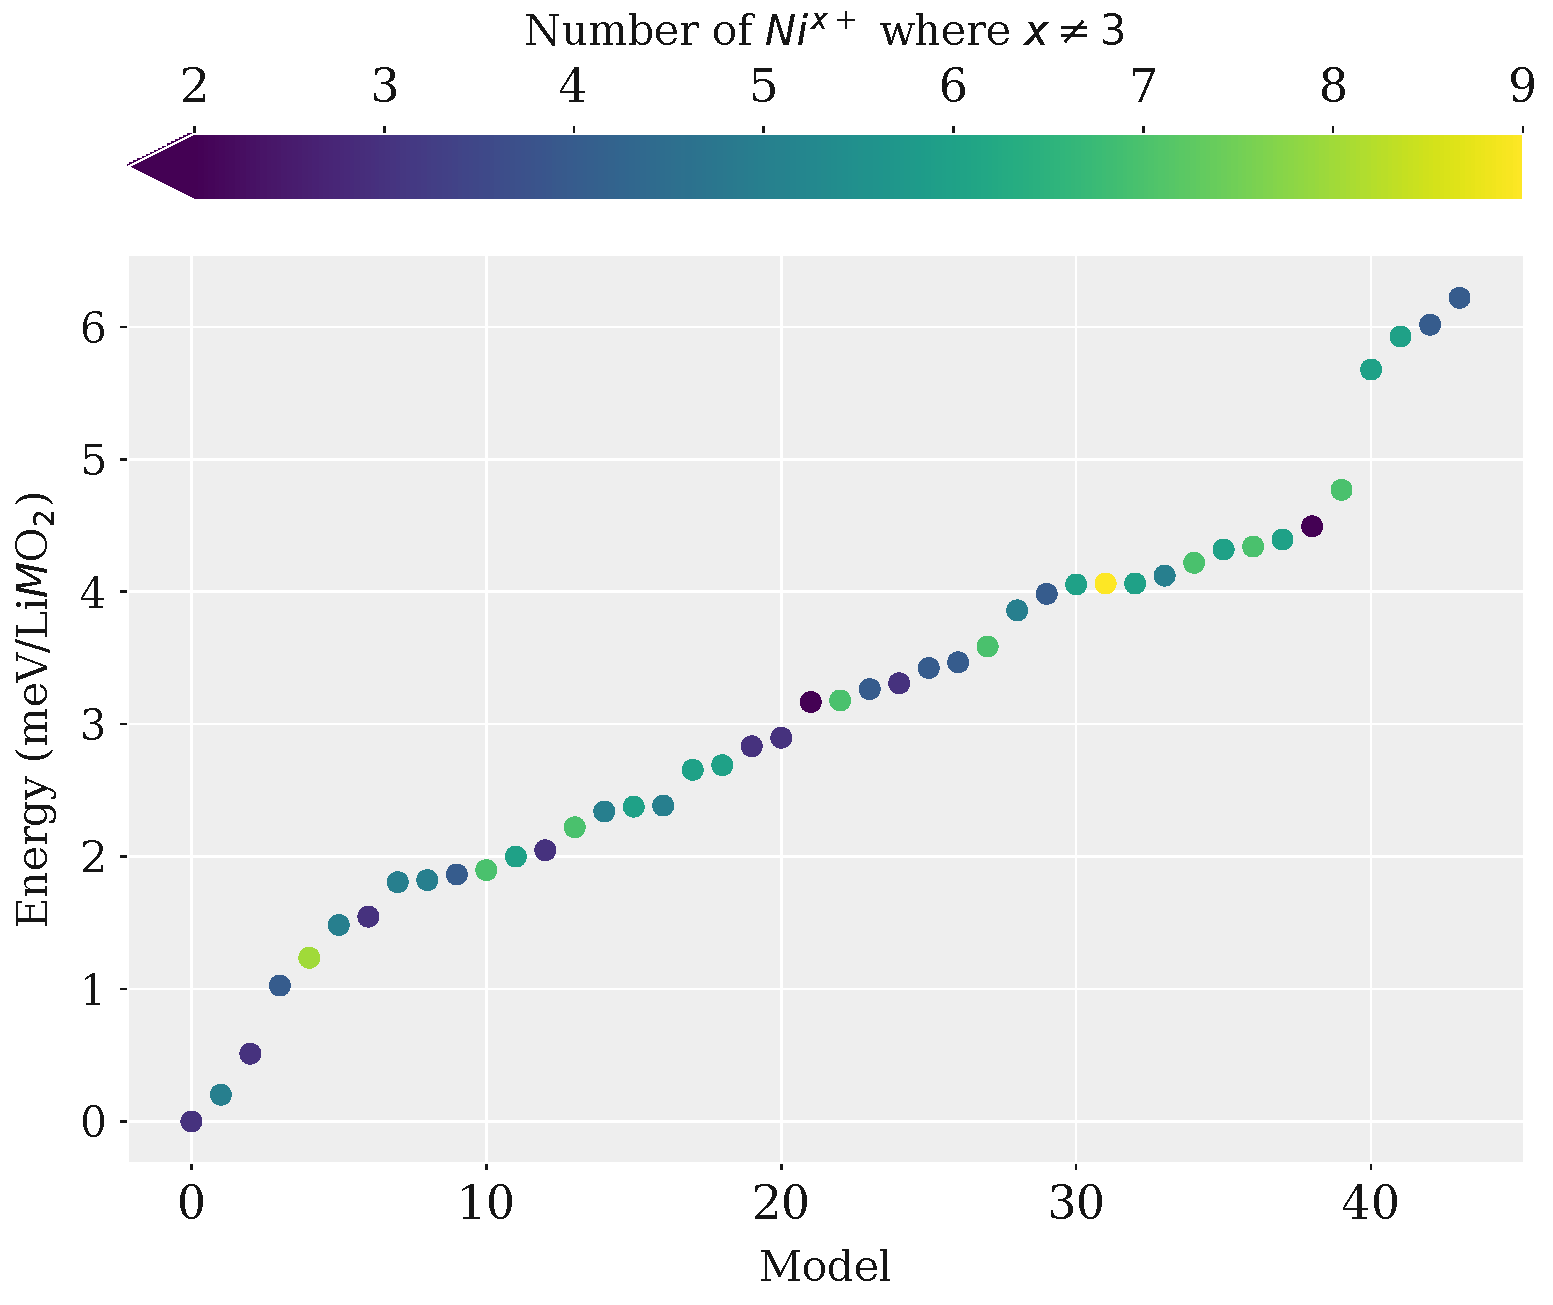
\includegraphics[width=0.46\columnwidth]{Figures/HSE_energy_cmap.pdf}&\includegraphics[width=0.46\columnwidth]{Figures/Ni_ox_vs_E.pdf}\\
  \textbf{(a)}&\textbf{(b)}\\
%    \includegraphics[width=0.75\columnwidth]{Ni_ox_vs_E.pdf}
   \end{tabular}
    \caption{\label{fig:stability} \textbf{(a)} Relative stabilities of different NMC-811 structural models obtained with the HSE06 functional, and the deviation in number of Ni$^{3+}$ in the material from the ``simple'' oxidation state model of \{1 Ni$^{2+}$;7 Ni$^{3+}$; 1 Mn$^{4+}$; 1 Co$^{3+}$\}, which would have 21 Ni$^{3+}$ for the supercell. \textbf{(b)} \% of Ni ion by oxidation state for each model, versus the relative energy per atom of the NMC model calculated with the HSE06 functional. Reproduced with permissions from \citenum{rana}. }
    \end{center}
\end{figure}

The analysis of the \% of Ni shows a mixture of Ni states, Figure \ref{fig:stability}(b). Nickel in NMC811 has been reported as having a mix of Ni(II/III) oxidation states, with the average value close to 3+, \cite{Zhu_JMatChemA2019,Kondrakov_JPhysChemC2017} which could potentially be rationalised by a simple distribution \{1 Ni$^{2+}$;7 Ni$^{3+}$;1 Mn$^{4+}$; 1 Co$^{3+}$\} oxidation state model. Several instances of this simple oxidation state distribution was found within \citeauthor{rana}'s data set. The two lowest energy structures here account for this oxidation state distribution. On examining the transition metal ordering in these lowest energy structures it can be seen that Mn$^{4+}$ and Ni$^{2+}$ lie in adjacent 3b sites along the shortest crystal axis. It forms continuous linear chains of alternating Mn$^{4+}$-Ni$^{2+}$ throughout all transition metal layers. This long range linear chain ordering is consistent with local charge balance, as discussed by \citeauthor{Zeng_ChemMater2007} \cite{Zeng_ChemMater2007}. As the two lowest energy structures contain this transition metal ordering, it suggests that the main stabilising effect of these models are the result of extended Mn$^{4+}$-Ni$^{2+}$ coordination. However, it should be noted that with the increase of supercell size, the probability of Mn$^{4+}$-Ni$^{2+}$ residing next to each other might reduce.

In a large proportion of NMC811 configurations \citeauthor{rana} investigated, $2$Ni$^{3+}\rightarrow$Ni$^{2+} + $Ni$^{4+}$ disproportionation is also observed. This occurs in some of the most stable structures in the data set, for example see the third most stable model in Figure \ref{fig:stability}(b). It can therefore be concluded that $2$Ni$^{3+}\rightarrow$Ni$^{2+} + $Ni$^{4+}$ disproportionation occurs in the pristine NMC811 structure before charging, illustrating that Ni$^{4+}$ is present in the fully lithiated material rather than only appearing on lithium deintercalation.

The finding from these studies are important for the improvement of electrochemical behaviour of cathodes as well as for the understanding of structural degradation of LIBs during cycling. Further studies on the effects of delithiation and doping on transition metal oxidation states currently underway to extend our understanding of NMC materials.

\section{Classical Molecular Dynamics Modelling of Diffusion Properties (Lucy)}
 \subsection{Interatomic Potentials}
DFT is well suited to investigate local hopping mechanisms such as Li diffusion in layered metal oxides by oxygen dumbbell hopping (ODH) or tetrahedral site hopping (TSH). \cite{van_der_ven_layered_2001, van_der_ven_LiTiS2_2008} When it comes to long range diffusion properties, however, classical Molecular Dynamics (MD) is better suited in terms of longer time- and length- scales. The atom interactions in classical MD are described using interatomic potentials. These can take multiple forms, each with different degrees of relevancy and accuracy depending on the system. Ionic solids, such as oxide systems including NMC, are widely described using a Coulomb-Buckingham potential, \cite{buckingham_classical_1938} derived from the Born model of the ionic solid \cite{born_1932, mayer_1932}, where the potential energy of the system is expressed as:

\begin{equation}
    E(r_{ij}) =  \sum_{ij} \frac{Q_i Q_j}{4\pi \varepsilon_0 r_{ij}} + \sum_{ij} A \ exp(\frac{-r_{ij}}{\rho}) - Cr_{ij}^{-6}
\end{equation}

Here, $i$ and $j$ are ions of charge $Q_i$ and $Q_j$ at a distance of $r_{ij}$ and $\varepsilon_0$ is the permittivity of free space. In the second term $A$, $\rho$, and $C$ are the parameters associated with the Buckingham potential.

An in depth exploration of literature reveals only a single classical MD study of NMC, where \citeauthor{Lee_and_Park_2012} employed core-shell Buckingham potentials for NMC111. \cite{Lee_and_Park_2012} Using these potentials for a range of NMC compositions, however, presented  catastrophic structural collapse upon removing Li (Figure \ref{fig:structure_collapse}). A sensical reasoning is Ni in NMC111 is Ni$^{2+}$, whereas in delithiated structures and other compositions, other oxidation states, such as Ni$^{3+}$ arise. Similarly, delithiation results in the formation of mixed Ni oxidation states and charge disproportion, which is challenging to represent in a classical model. \cite{Nakamura_2019,Kim_2002,Alonso_1999} The complex nature of Ni chemistry extends to the LiNiO$_2$ ternary system. To the best of our knowledge, no interatomic potentials exist for Ni$^{3+}$, evidenced by a lack of classical MD publications for LiNiO$_2$ and NMC systems. Development of new interatomic potentials for the LiNiO$_2$ and NMC systems, was therefore necessary.

\begin{figure}[h]
  \centering
  \resizebox{8cm}{!}{\includegraphics*{Figures/structure_collapse.pdf}} %
    \caption{\label{fig:structure_collapse} Structure images for fully lithiated (centre) and 20 \% delithiated (right) NMC811 after an initial equilibration MD simulation using potentials from \citeauthor{Lee_and_Park_2012} (left). \cite{Lee_and_Park_2012} }
\end{figure}

\subsection{Developing Interatomic Potentials}
For layered structures, variations of the Buckingham potentials are presented in literature: Some using rigid ion models,\cite{Lewis_1985, Ledwaba2020, Sayle2005, Dawson2014} with others using core-shell models, \cite{Hart1998, Fisher2010, Lewis_1985,Ammundsen1999, Kerisit2014, He2019,lee2012atomistic} with a mixture of formal and partial charges. As literature is in disagreement over most representative variation of the Buckingham potential, fitting and comparing different permutations of the Buckingham potential is needed. Interatomic potentials are most commonly based on mathematical functions parameterised using experimental and/or ab-initio derived data. \cite{jones_1924, buckingham_classical_1938} A limited number of codes are available with the functionality to fit classical potentials, including the general utility lattice program (GULP), \cite{gale_gulp_1997} Atomicrex, \cite{Stukowski_2017} dftfit, \cite{dftfit} and potfit. \cite{wen_kim-compliant_2017} These codes poses individual features, however, none were able to accurately produce potentials for NMC or LiNiO$_2$, with only GULP having the capability of fitting core-shell models.

\re{Buckfit}, \re{ add citation\cite{}} a code developed within the Faraday institution, was specifically created for fitting different permutations of the Buckingham potential. Its modular design allows flexible fitting of both rigid ion and core-shell models, and formal and partial charges. Here, we review important aspects determined to be vital when fitting potentials for NMC and LiNiO$_2$, using the \re{Buckfit} code to isolate individual features and the resulting effects on the \textit{fit} of the potential.

In systems such as NMC and LiNiO$_2$ the short-range interactions are overwhelmed by the longer-range coulombic term. In these cases, the system charges need to be scaled down to increase the influence of the short-range interactions, termed as partial charges. A scaling factor of 60 \% formal charge is commonly used, \cite{pedone2006potentials} however, partial charges are to some extent system dependant. Figure \ref{fig:charge_scaling} shows $\chi^2$ (fit error) for a fitted Buckingham potential for LiNiO$_2$ reduces with the charge scaling factor until approximately 60 \% of the formal charge, where it starts to plateau. This is in broad agreement with literature, with a slightly improved fit at $\sim$50 \% formal charge.

\begin{figure}[h]
    \centering
    \resizebox{7cm}{!}{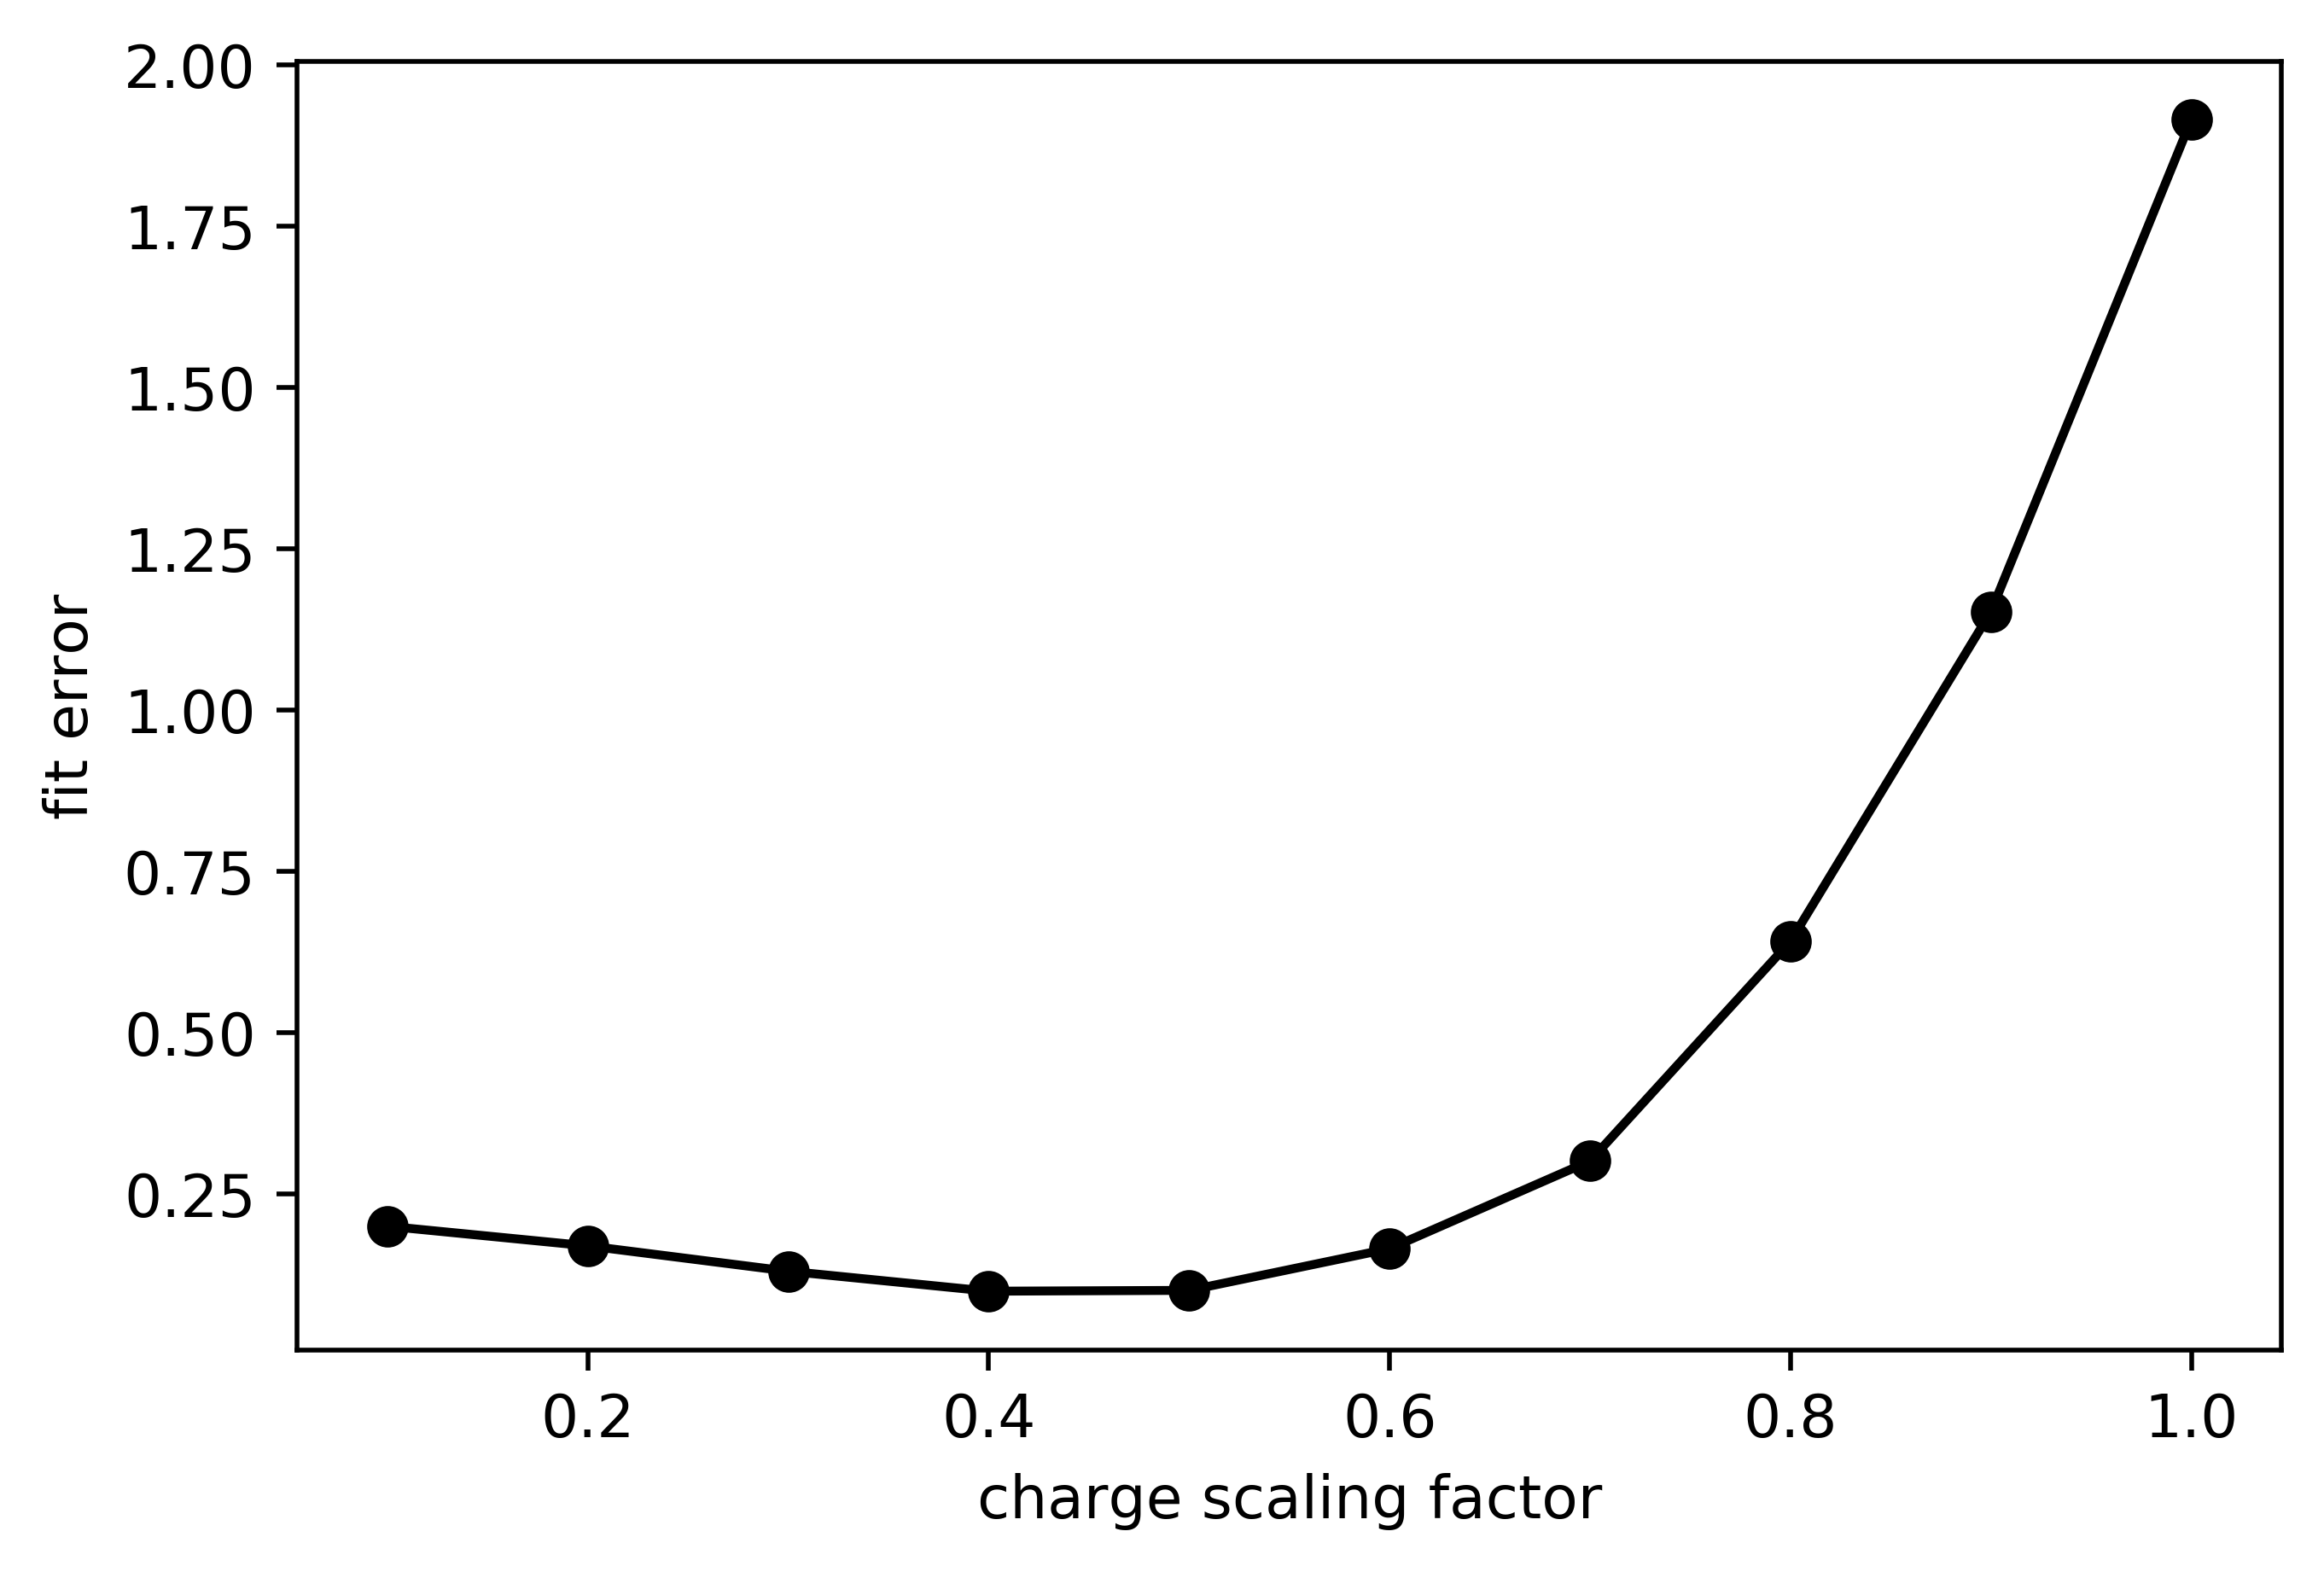
\includegraphics{Figures/charge_scaling_error_plot.png}}
    \caption{\label{fig:charge_scaling} Plot of the fit error (mean squared error, $\chi^2$) of LiNiO$_2$ as a function of the charge scaling factor.}
\end{figure}

Core-shell models introduce polarizability into classical MD simulations. The adiabatic shell model \cite{Mitchell_1993} is widely used in literature \cite{Hart1998, Fisher2010, Lewis_1985,Ammundsen1999, Kerisit2014, He2019,lee2012atomistic} for calculating long trajectories. A fraction of the atomic mass is assigned to the shell and there is no explicitly defined fraction size; however, placing 10 \% of the atomic mass on the shell is commonly adopted. \cite{PLIMPTON19951,todorov2006dl_poly_3} An additional consideration is the separation of the formal atomic charge across the core and shell. However, determined numerical values of the core-shell charge separation are inconsistent. \cite{wang2014molecular,escribano2017enhancing,lee2012atomistic,Lee2013_lithium,dai2019comparison}

Fitting a fully rigid ion potentials for LiNiO$_2$ (with partial charges) resulted with a best fit of $\chi^2$ = 1.665, however introducing a core-shell potential on the oxygen, with Li and Ni remaining rigid ion, $\chi^2$ was reduced to 0.372. Presenting evidence that a core-shell potential is required to more accurately reproduce the forces and physics of the system. In the case of the oxygen core-shell the spring constant was determined to be 15.443 eV $\cdot$\AA$^{-2}$, with a charge of -1.48 e on the shell and 0.520 e on the core.

Here, the best fit (lowest mean squared error) was a core-shell model on the oxygen in a partial charged system. The resulting potential was used with a 10 \% delithiated LiNiO$_2$ supercell to conduct MD studies at 700 K on the diffusion within the material. The MSD, Figure \ref{fig:MSD_LiNiO2}, presents a fairly small movement of the lithium atoms, however the resulting self-diffusion coefficient, 6.664$\times 10^{-8}$  cm$^{2}$ s$^{-1}$, is within the range measured experimentally. \cite{Nakamura2000}

\begin{figure}
    \centering
    \resizebox{7cm}{!}{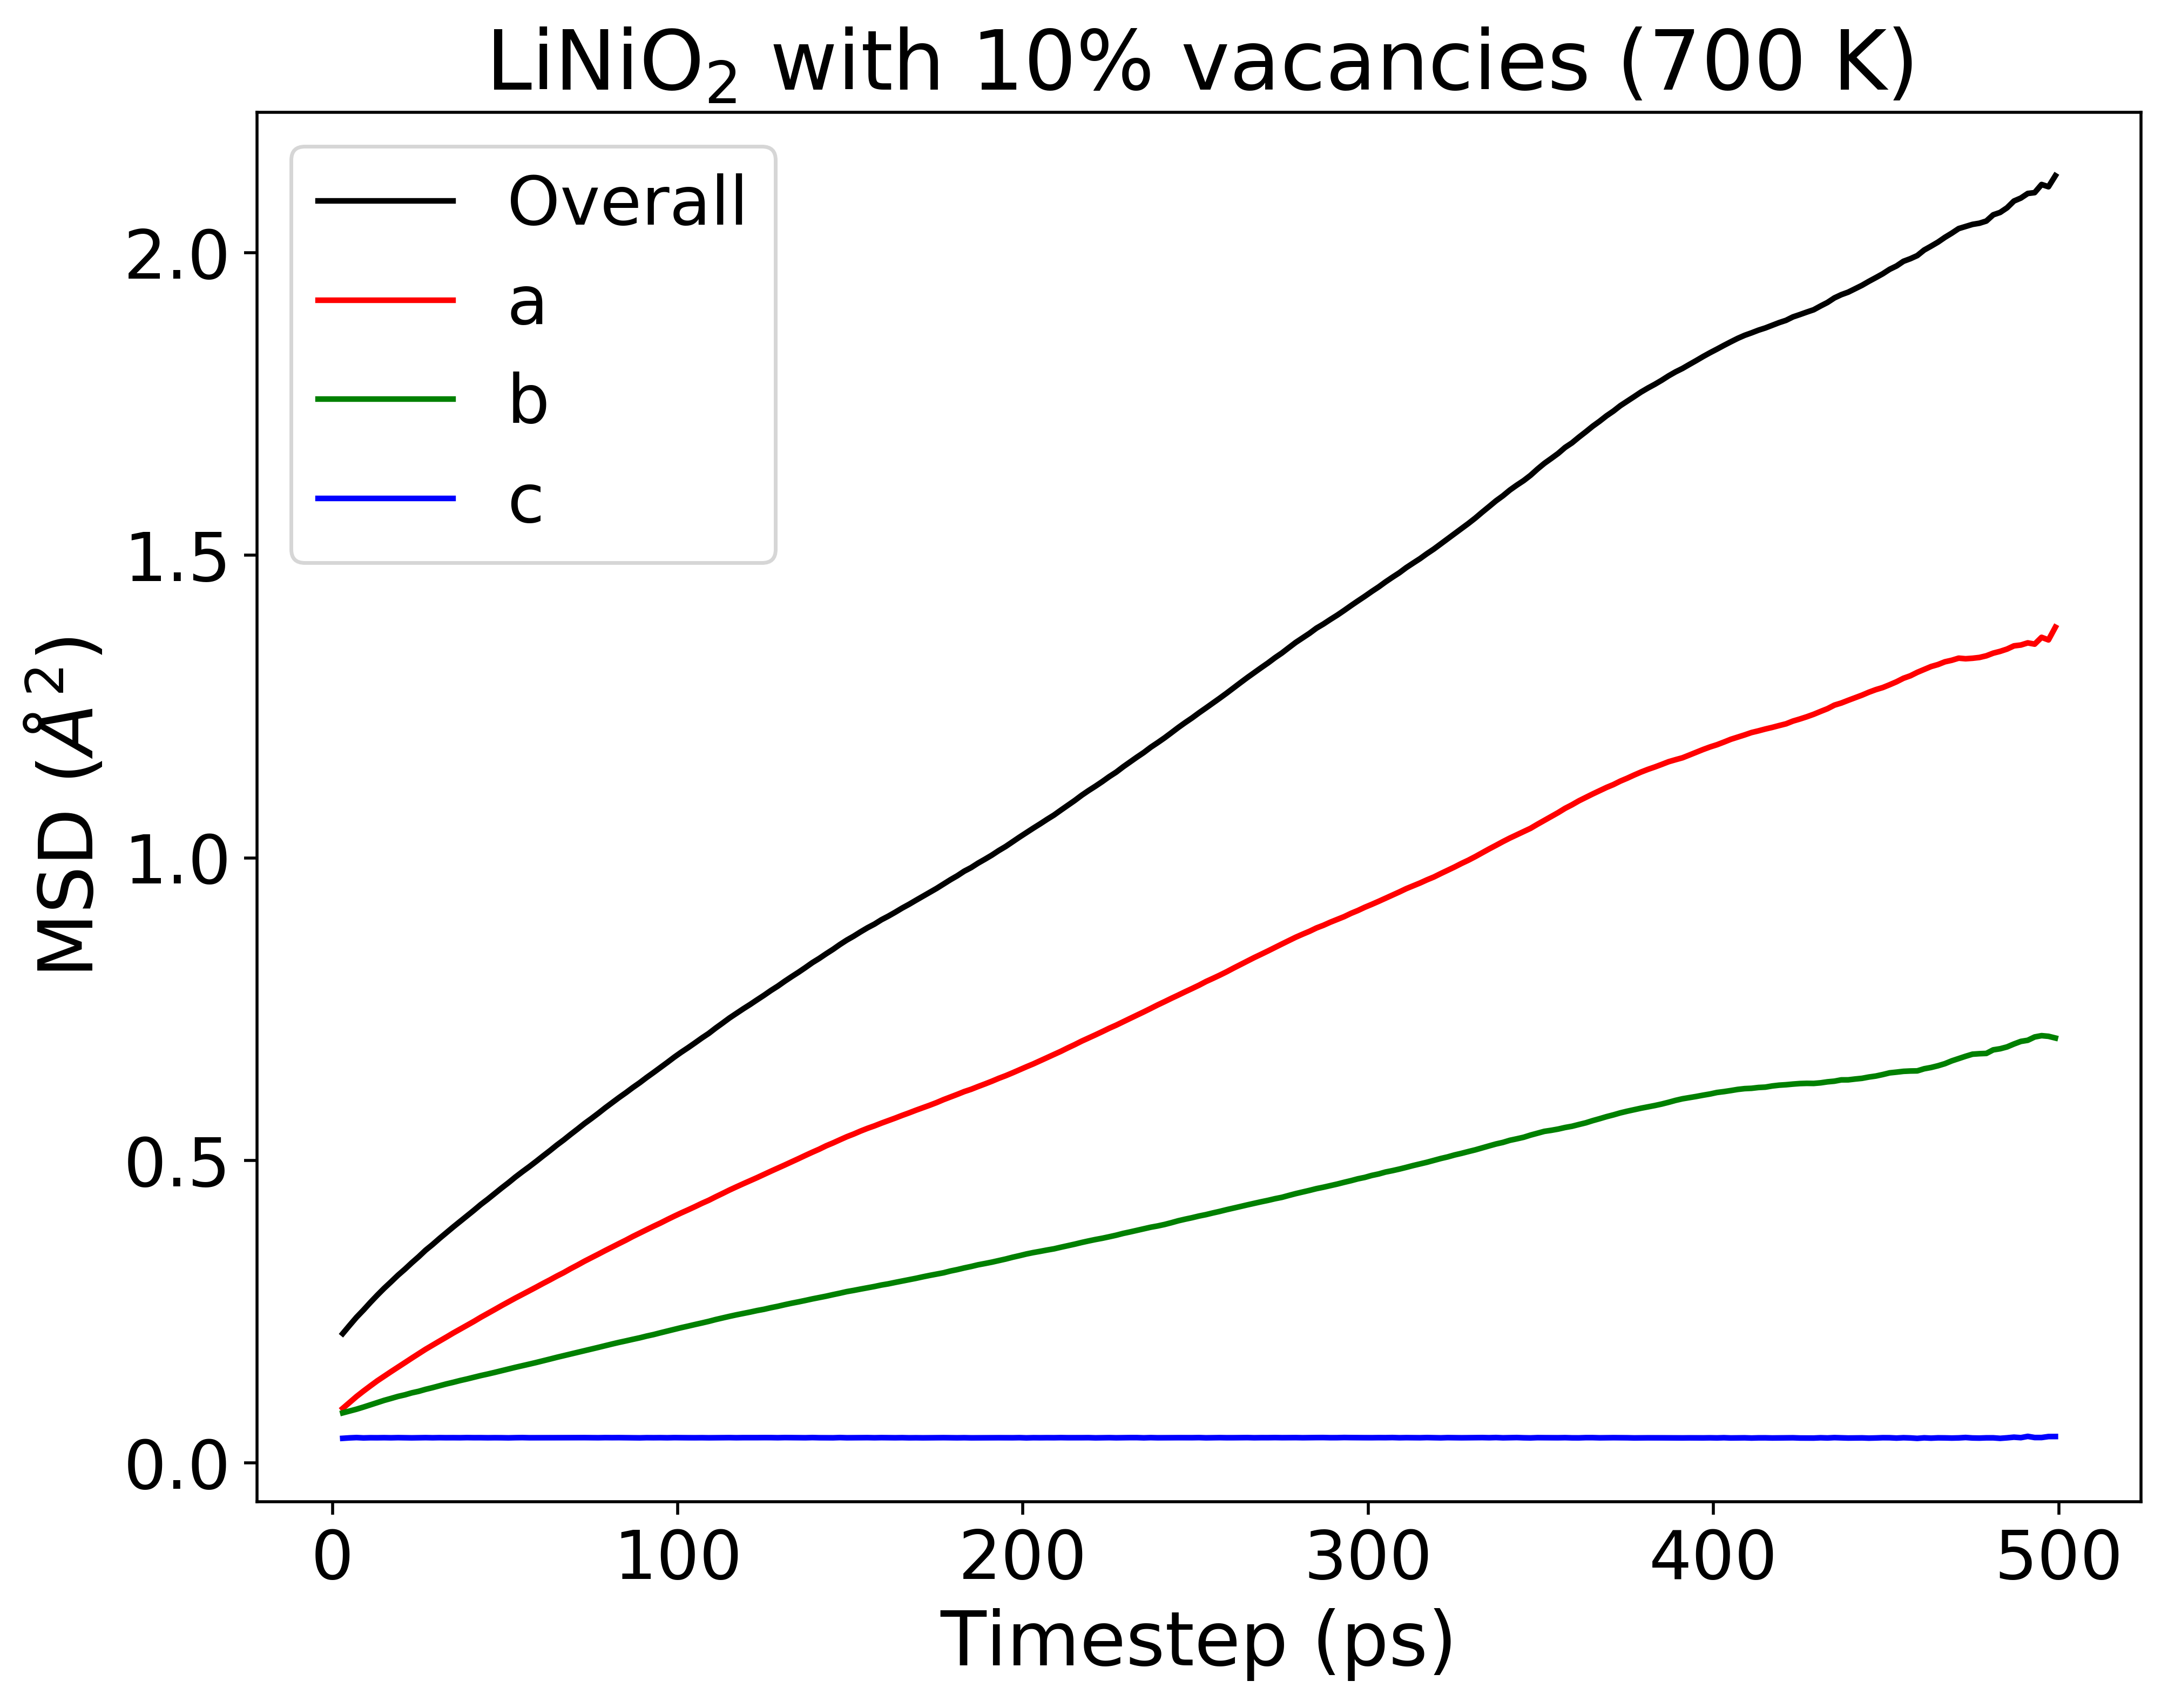
\includegraphics{Figures/MSD_LiNiO2.png}}
    \caption{\label{fig:MSD_LiNiO2} Plot of the mean squared displacement (MSD) of Li in LiNiO$_2$ with 10 \% Li vacancies at 700 K. As this is a layered material, it is expected that no movement will occur in the c direction, only in a and b.}
\end{figure}

These results indicate that to get the best fit for the interatomic potential, core-shell and partial charges must be included, however, although the MD presents diffusion within the experimental range for the material, the diffusion is so low that it is indistinguishable from in-place vibrations on this timescale. Further validations are needed to determine whether this particular potential is adequate to represent the physics in the system, however, it highlights the considerations needed for this class of material.







\section{Parameterisation \& Continuum Modelling (Kieran)}

\subsection{Introduction}
Beyond the crystal lattice, the properties of which are governed by atomistic behaviour, continuum models simulate the behaviour of a battery at cell level. Connecting continuum and atomistic models predictions would provide better understanding of the charge and mass transport processes, resulting in better predictions of battery behaviour. These models are governed by mathematical expressions that relate concentrations and potentials. Atomistic theory considers every individual particle, whereas continuum models consider an average following the continuum approximation (Ref).  The values required for these models can be constants or variables, these inputs are known as parameters. Attempts to couple these scales have shown that there is no sound mathematical way to link them.\cite{Fackeldey2015} The respective governing equations are different: continuum models comprise of partial differential equations (PDEs) and atomistic models are discrete models.\cite{Badia2007} This means they depend on unique parameter sets. For example, atomistic charge transport relates to self-diffusion in the crystal lattice, whereas at the continuum scale this process relates to macroscopic diffusion within the electrode, often being experimentally determined.

In battery research the most commonly used continuum model is the Doyle-Fuller-Newman (DFN) model.\cite{Newman1975porous, Doyle1993DFN} The DFN model is an electrochemistry-based model that predicts the dynamics of a battery based on concentrations and potentials. The DFN model requires over 25 parameters with the exact number depending on how the equations are expressed.\cite{Kim2011} Parameter estimation can be used, but the process is complicated by the large number of parameters.\cite{Jin2018} The favoured approach to parameterise a battery model involves the use of various experimental techniques.

The computational expense of the DFN model precludes their use in battery management systems, and equivalent circuit models are favoured due to their simplicity.\cite{Marquis2019} However, once parametrised, the DFN model can be used in battery material development by providing more detailed physical insight compared to other model classes.\cite{Dawson2018} Recent interest in Ni-rich cathode materials has seen the DFN model used extensively to understand the use of graded electrodes (containing multiple electrode particle sizes), to deconvolute capacity and power fade predictions, and to investigate the efficacy of tab and electrode designs for fast charging.\cite{Richardson2020,Kindermann2017,Sturm2019} This research has been dependent on parameter sets for NMC materials being reported, however, these values may not reliably describe the properties of Ni-rich NMC because studies may use parameters determined for cathodes with lower Ni content. In this section, we report the significance of parameterisation in model development and how these developments contribute towards widening the applications and improving the performance of Ni-rich NMC cathodes, primarily NMC811. Furthermore, we highlight several parameterisation efforts investigating the physico-electrochemical and thermal properties to gain new insights and the availability of software that increases accessibility to these parameters enabling better research. 

\subsection{Procedures, Properties, and Packages}
\subsubsection{Procedures}
The parameterisation methods are developed using a lithium-ion battery with a specific chemistry and format, but these methods are agnostic i.e. techniques demonstrated on one battery can be applied to many others. The parameters in the DFN model describe the physical, chemical, and electrochemical properties of a battery. Evaluating these properties requires a suite of experimental techniques. These techniques include imaging, bulk/surface chemical methods, electrochemical characterisation, and electrolyte analysis (Figure \ref{fig:param_pie}). \cite{Waldmann2016} It is important to be aware of the limitations in parameter values, both due to the techniques and how these values are reported. The latter concerns the fact that these parameters are often reported as constants but are significantly dependent on state of charge and the parameters relate to a specific battery comprised of unique materials. Multiple techniques can be used to determine each parameter, the choice of technique influences the reported value as each has shortcomings. Several papers compare the parameter values obtained for tortuosity, composition, open-circuit voltages, and electrode microstructure for different techniques. \cite{Nguyen2020,Chen2020, Landesfeind2018, Barai2019} These comparisons provide a robust approach as the certainty of parameter values is better illustrated. However, the technique chosen is often due to the availability of equipment and relevant expertise, rather than providing the most robust approach.

\begin{figure}[h]
    \centering
    \resizebox{8cm}{!}{\includegraphics*{Figures/param_pie.png}} %
    \caption{\label{fig:param_pie} Diagram of the techniques used to parameterise the behaviours of NMC811. [Include DFN symbols]} 
\end{figure}

In many modelling experiments, parameters are collated from various literature sources.\cite{Kim2011} This process almost always consists of assumed and/or fitted parameters such as electrode geometry, diffusion coefficients, and activation energies.\cite{Merla2018} The active material and electrodes have purposefully designed compositions and morphologies depending on application, these factors significantly influence the resulting properties.\cite{Lain2019} Simulations using parameters obtained from literature sources prove less accurate because the values do not adequately describe the cell being investigated.\cite{Zhang2014} The parameters measured may be suitable for a specific cell, therefore for different cell chemistries the parameters will have to be reevaluated. For NMC811 the diffusion can vary over orders of magnitude.\cite{Kim2011,noh2013comparison} This difference can be attributed to differences in composition, particle morphology, and electrode geometry.\cite{Liu2008,Luo_2015,Michaelis_2019_understanding} It is not suitable to regard a battery as a "blackbox" with properties being reliably described by literature values, but rather to determine them through tear-down and postmortem characterisation. This process is time consuming and research-intensive, however it provides the most robust approach to provide models with appropriate inputs. 

\subsubsection{Properties}
Transitioning to higher Ni contents in layered oxide materials is essential to increasing the energy density of cathode.\cite{Li_Erickson_Manthiram_2020, Manthiram_2020} The trend to increase nickel content in NMC has been motivated by improving range in electric vehicles and the ethical implications of cobalt mining. \cite{Nkulu2018,Banza2009} Commercialising high-nickel oxides is dependent on developments in their compositional, morphological and microstructural design. Parameterisation is essential for modelling these materials, as simulations act as a powerful tool to investigate the properties and of NMC and optimise design without the need to conduct resource-intensive experiments.\cite{shearing_2020_3D} 

Previously, several NMC-based (with low nickel content) batteries have been experimentally parameterised. \cite{Ecker2015,Schmalstieg_Rahe_Ecker_Sauer_2018,Liebig_2019}  \citeauthor{Ecker2015} reported the physico-chemical properties and anatomy of a LiNi$_{0.4}$Co$_{0.6}$O$_2$ based pouch cell, offering a comparison of the efficacy of different techniques used to evaluate the kinetics. \cite{Ecker2015} \citeauthor{Schmalstieg_Rahe_Ecker_Sauer_2018} investigated a battery composed of a LiNi$_{0.33}$Mn$_{0.33}$Co$_{0.33}$O$_2$ mapping many of the parameters as a function of lithiation, and defining the stoichiometries of each electrode. \cite{Schmalstieg_Rahe_Ecker_Sauer_2018} \citeauthor{Liebig_2019} studied the electrochemical behaviour of a large format NMC cell, extending the model parameterisation and predictions to include thermal behaviour. \cite{Liebig_2019}  These papers outline parameter sets that can be used in simulations and the methodologies used to determine them. These parameterisation strategies prove a valuable tool for other groups to undertake similar investigations, by detailing a procedure that can be applied to other materials. However, for modellers investigating the behaviour of high-Ni NMC materials these parameters provide limited utility as they do not accurately describe the properties. This can be attributed to the electrochemical properties being significantly affected by the stoichiometric ratios in NMC materials.\cite{noh2013comparison} 

It is difficult to predict the values of parameters for high-Ni materials based on the determined values for lower Ni-content materials.\cite{Amin_Chiang_2016} This is attributed to the presence of different thermodynamic phases compared to NMC811, which affects the dependency of several parameters on the state of lithiation. \cite{jung2017oxygen} To address the limited contributions in this context, authors have focused on specifically parameterising NMC811 chemistries. \citeauthor{Chen2020} detailed the parameters for a 21700-cylindrical cell, validating and tuning these values for cell discharge.\cite{Chen2020}  Sturm \& Jossen \textit{et al.} provided a full electrochemical-parameterisation of a DFN model to study lithium plating during fast charging in a NMC-811/SiC cell. \cite{Jossen2019,Sturm2019} It can be time consuming to conduct literature searches to find parameters, to develop the code to simulate battery behaviour, and to collect the data to validate model predictions. The availability of software and data has been essential in enabling innovations in this field.

\subsubsection{Packages}
Traditionally, the sourcing of parameters required an extensive literature search and/or knowledge of prominent authors in the field. Recently, the development of databases and software that collate parameter values for battery components have streamlined this process and proved essential in modelling applications.\cite{Tranter2020}  Wang et al. created a database that details over 100 parameterisations of batteries or the individual components and the techniques that have been used to determine them. These entries are dominated by NMC-chemistries due to the commercial relevance, but there are many entries that characterise separators and electrolytes. Additionally, Python Battery Mathematical Modelling (PyBaMM) is a software package that has been explicitly developed for continuum modelling, it caters for multiple definitions and allows the construction of a battery from electrodes and an electrolyte that have been parameterised.(37-PyBaMM) There are several electrode chemistries and electrolyte systems currently available, this list is expanding as users add new sets. PyBaMM contains a parameter set for an NMC811 electrode, this is denoted by the label "Chen2020".\cite{Chen2020} This parameter set has been utilised in several investigations.\cite{Tranter2020} PyBaMM provides a robust approach to modelling of NMC chemistries as the electrochemical behaviour can be simulated with only several lines of code (Figure \ref{fig:pybamm}).

Furthermore, validating model predictions requires data from electrochemical experiments or from electrode imaging.(ref) Data repositories provide researchers with access to the required data, removing the need for researchers to conduct experiments they do not have the required expertise or equipment for. Recent pressure for data availability in science, providing parameter values and raw data improved accessibility and transparency leading to better research. \citeauthor{Ebner_Geldmacher_Marone_Stampanoni_Wood_2013} have provided the tomographic data (raw and processed) and the corresponding electrochemical data for 16 different LiNi$_{0.33}$Mn$_{0.33}$Co$_{0.33}$O$_{2}$ cathodes. \cite{Ebner_Geldmacher_Marone_Stampanoni_Wood_2013} \citeauthor{Chen2020} have made available data on the discharge and subsequent relaxation of the NMC811-based cylindrical cell that was used in the validation of the parameter set  (Ref. \citenum{zenodo}). \cite{Chen2020} \citeauthor{Devie_2018} have provided datasets on the degradation of 18650 cylindrical cells based on NMC, NCA, and LFP chemistries, the study is ongoing and is examining the influence of temperature (depth of discharge), and discharge (current) on the ageing of cells (Ref. \citenum{BatteryArchive}). \cite{Devie_2018} 

\begin{figure}[h]
    \centering
    \resizebox{8cm}{!}{\includegraphics*{Figures/pybamm.png}} %
    \caption{\label{fig:pybamm} PyBaMM simulation} 
\end{figure}

\subsection{Conclusions}
Parameterisations are a critical exercise in model development, additionally they provide useful insights into the properties of a lithium-ion battery and its components. It is important to be aware of the nuances in reported parameter values, specifically that different techniques provide considerably different information and that modelling predictions are most accurate when the parameters have been explicitly determined for the battery being studied. The availability of parameters and validation data has proven valuable to the research community, software has been developed in this context. For example, PyBaMM has is a powerful tool that connects researchers with parameter sets and robust code.  

The thermal and electrochemical behaviours of battery materials have been widely described, however, being able to accurately predict the degradation has proven more difficult. This can be ascribed to the difficulty measuring the required parameters, presently, many of these parameters are assumed or fitted. 


\section{Degradation Processes Effecting NMC811 and Experimental Approaches to Identifying and Monitoring (Anisha)}

\subsection{Introduction}
Current applications for LIBs demand fast charging and high energy density from batteries, the ability of a battery to perform to these requirements is highly dependant on the cathode material and the transition metals they are composed from.\cite{Sari2019, Julien2014} High energy dense cathode materials have intrinsic limitations that lead to degradation, this is accelerated by fast charging.\cite{Xia2018} These processes need to be understood to build  models that can accurately predict lifetime, as well as developing these materials to meet performance requirements.\cite{Hendricks2015} NMC is a three component cathode material that combines the merits of three transition metals; the high capacity from nickel, the thermal stability from manganese, and stable electrochemical characteristics provided from cobalt. Each of these cations and their chemistries contribute differently to the performance of a battery and to the degradation mechanisms.\cite{Julien2014}
The steady increase in the Ni content has resulted in different generations of NMC material, ranging from stoichiometries of NMC111 to NMC811 all of which with increasing capacity.\cite{Sari2019} 

\subsection{Key Degradation Mechanisms}
Cathode materials undergo two key degradation modes: loss of lithium inventory (LLI), loss of active material (LAM) and changes in impedance caused by a range of physical and chemical mechanisms, which effects the cells overall power and capacity fade. These mechanisms include interactions between the electrolyte and the highly reactive delithiated cathode surface at high potentials. The disadvantages of moving towards higher nickel content is the increase in parasitic reactions that accelerates different degradation modes,  such as active material degradation or dissolution, phase transition, oxygen release, and cation mixing.\cite{Dixit2017}     


At high voltages, high-Ni NMC structures become thermodynamically unstable and oxidation of the electrolyte at the cathode electrolyte interface (CEI) takes place, resulting in a passive layer which consumes Li ions and increases impedance. Repeated charge-discharge cycling is a leading cause of mechanical degradation in the electrode materials and in the CEI due to substantial structural and volume changes during lithiation and delithiation. This results in particle cracking \cite{Woodford2010} and loss of contact between particles and current collector.\cite{erickson2017recent} Although, the cracks become filled by electrolyte, which results in an increased active surface area and charge transfer kinetics leading to further uncontrolled side reactions with electrolyte, hence increases CEI formation and LLI.\cite{erickson2017recent}

In addition, the highly oxidised nickel cations react with the electrolyte, leading to transition metal (TM) dissolution.  

The high reactivity of non-aqueous organic electrolytes with water means any trace contamination of moisture will result in electrolyte decomposition and the production of HF that goes on to attack the cathode material leading to LAM.\cite{Zheng2012} 

These dissolved TM ions can further react with electrolyte forming precipitates that redeposit on to the cathode interface, increasing the CEI layer and further increasing impedance.\cite{Zheng2012} 

Cation mixing takes place when Li$^{+}$-Ni$^{2+}$ site mixing occurs. During this phenomenon, Ni$^{2+}$ changes its position within the NMC crystal lattice to the Li$^{+}$ site, this impedes Li$^{+}$ diffusion back into the cathode.\cite{Sari2019} Increasing the nickel content promotes this phenomenon as well as increases parasitic reactions that accelerate different degradation modes.\cite{erickson2017recent} 

Monitoring the degradation state and understanding the processes taking place within a cell aides in managing capacity fade and protecting cell from early failure such as thermal runaway, by predicting behaviour and management to ensure appropriate use of an already aging cell as to avoid accelerating degradation. Battery management systems (BMS) monitor  state of health (SoH) by estimating capacity and internal resistance. In order to use models to estimate aging mechanisms during normal or even fast charging, accurate determination of the parameters that describe the physical, chemical, and electrochemical properties of the cell is key. The reliability of models to predict a cells behaviour, which varies between different types of cells, requires experimental data.

\subsection{Experimental Techniques}
A range of electrochemical techniques are used as non-invasive diagnostic tools to characterise a cells SoH, providing information on the capacity loss and resistance change, as well as aiding diagnosis of the underlying processes taking place. Degradation is affected by the operating conditions such as temperature, load current, and state-of-charge (SOC). Electrochemical techniques using galvanostatic and potentiometric control are standard approaches to determine cell voltage and total capacity within a voltage range from it’s beginning of life (BoL) to it’s end of life (EoL). The most practical approach to assessing capacity, reversibility, stability and rate capability involves charging the cell by maintaining a constant current (CC) until the cell reaches a defined voltage limit, then holding the cell at a constant voltage (CV) step within a defined period of time and to a current limit. Discharge steps involve a CC step, which is sometimes  followed by CV step, and always has rest periods before and after. The resulting capacity of a cell is dependant on temperature, hence measurements are carried out under temperature control, and the reversibility of resulting charge and discharge curves provide information on the changes in LLI and LAM.\cite{Birkl2017}

Open circuit voltage (OCV) experiments measure the equilibrium voltage of a cell and relate to the batteries state of charge (SoC), providing thermodynamic information such as phase transitions from Li$^{+}$ intercalation and deintercalation. The OCV of a LIB is affected by aging, and therefore used for diagnosis of SoH. Tests can be carried out in a full cell, where the curve is defined by both the cathode and anode, or in a half cell, where one electrode is measured against a reference, and is typically obtained from a pseudo-OCV curves or Galvanostatic intermittent titration technique (GITT).It should be noted that when using pseudo-OCV for modelling, the charge and discharge hysteresis needs to be taken into consideration.\cite{Garcia-Plaza2017} 

Pseudo-OCV tests are the same as capacity experiments but where the current rate is slow enough (e.g. from C/20 to C/33) in order to minimise kinetic contributions, electrode polarisation and ohmic heat generation, allowing thermodynamic processes dominate.\cite{Bloom2005} Advanced electrochemical analysis that can be carried out from pseudo-OCV data for differential voltage (DV) and incremental capacity (IC) analysis, which produce plots with peaks at specific voltages that correspond to cell chemistry, such as phase transitions and redox processes taking place in the cathode as well as LLI.\cite{Bloom2005} Integrating the area under peaks and comparing the ratio for subsequent cycles provides information on which processes are dominating, fading or unaffected by the cycling. Shifts in peak position correspond to changes in impedance for the corresponding process, providing information on which processes are becoming more resistive, and are useful to monitor from BoL as the cell ages.\cite{Barai2019} 

GITT involves a series of current pulses and relaxation steps to fully discharge or fully charge a cell, during which the cell potential is measured.\cite{Dees2009} The technique is based on several underlying assumptions, which should be verified in order to confirm applicability.\cite{Dees2009} During the relaxation step, the Li ion distribution in the electrode homogenises and is dependent on the cell temperature. Lithium ion diffusion coefficients can be extracted from test using models such as the pseudo-2D model proposed by Doyle, Fuller, and Newman. \cite{Doyle1993DFN} This approach avoids kinetic contributions and considered to be most reliable for obtaining OCV data, however it requires long relaxation periods, at least four hours, between steps meaning tests take several weeks to complete. In contrast, pseudo-OCV is more practical to carry out than GITT test and has the added benefit of DV and IC characterisation. Both extract thermodynamic information on transition metals of the cathode and anode undergoing lithiation and delithiation.

Electrochemical impedance spectroscopy (EIS) is advanced analysis to investigate cell impedance and investigate fundamental electrochemical dynamics. The technique is based measuring the response of a cell to a small AC sinusoidal voltage or current, resulting in amplitude and phase shift of the cells response is measured across a frequency range. The dependency of EIS on SOC or temperature is usually characterised.\cite{Andre2011} The resulting EIS data is most commonly analysed using the Nyquist plot, composed of the real part the impedance on the x-axis and the imaginary on the y-axis, sections of this plot is related to different parts or processes inside the cell and the shape of the Nyquist plot is representative of the electrochemical processes at the surface of the electrodes, such as the CEI, processes in the bulk of the electrolyte, such as lithium ion diffusion, as well as LAM, and phase or structural changes within material.\cite{Jalkanen2015, Andre2011}
The Bode plot the phase shift is related to the electrochemical and transport processes, which is not evident from the Nyquist plot. Mathematical models based on kinetic and transport equations, e.g. equivalent circuits, are used for interpreting data and require estimates of parameters, therefore often challenging and ambiguous. EIS tends to be carried out alongside other techniques for a more comprehensive investigation, for example, with GITT, periodically within capacity fade, followed by invasive material characterisation. \cite{Jalkanen2015}

Complementary data can be obtained from physico-chemical characterisation, which further enhances our understanding of processes taking place during charging and discharging, and  provides further parameters to support the development of realistic and improve accuracy. This type of characterisation is generally destructive, requiring teardown of cells at various points during cycle ageing for analysis. Microscopy techniques, such as optical, scanning electron microscopy and transmission electron microscopy, are used to characterise the structural changes e.g.  porosity, particle size and cracking, X-ray and spectroscopic techniques are used to access chemical composition, including lithiation of NMC particles and the CEI layer.\cite{Waldmann2016} Some in situ techniques have been successfully demonstrated to reveal important microstructural and chemical information, for example, X-ray diffraction computed tomography was carried out on a full cell during operation to study the crystal dimension changes in NMC material.\cite{Sohrab2020} The use of multiple techniques to characterise NMC cells  produce the most comprehensive analysis. Dahn et al investigated the effect of high voltage on cycling performance at voltage using microscopy, ex situ and in situ X-ray characterisation, as well as calorimetry to supplement electrochemical data. The group found a dramatic change in active material at high voltages as well as parasitic reactions between the electrolyte and the highly delithiated NMC811 to be the cause of failure at potentials above 4.2V.\cite{Li2015} 

\subsection{Conclusion}
Key degradation processes that take place at the cathode material and their effects have been discussed, and fundamental characterisation techniques that aide tracking and monitoring of these processes have been introduced. Electrochemical techniques are fast and practical diagnostic tools used in situ characterisation of battery performance, providing information on capacity, resistance and coulombic efficiency. The use of multiple approaches produces rich data, which is required for cell monitoring, deciphering the degradation processes taking place during cell cycling, and essential for accurate parameterisation and validation of models, leading towards the design of more realistic models for accurate prediction of cells life.

\section{Continuum Modelling (Abir)}
Increasing commercialization of high-Ni layered lithium nickel manganese cobalt oxide (LiNi$_x$Mn$_y$Co$_z$O$_2$, NMC) positive electrodes (PEs) necessitates degradation studies on  these materials. The study of degradation mechanisms is important to make knowledge available for the battery manufacturers to produce Li-ion batteries with higher specific capacity at a significantly lower cost. \cite{du2020battery,jaguemont2016comprehensive} Among the other variants of high-Ni NMC structures, NMC811 PEs provide higher reversible capacity because a higher number of Li-ions can be extracted during operation within the same voltage window. \cite{andre2015future,noh2013comparison} However, NMC811 structures are not stable when an exceedingly large fraction of Li-ion is removed during charging of the cell and the structures lose their retained capacity easily. \cite{gabrisch2008transmission,liu2015nickel}

The chemical and mechanical degradation processes the NMC electrode material undergoes has been introduced.The parasitic degradation processes TM dissolution, CEI, and oxygen evolution, introduced above,  are important features of chemical degradation in NMC and can be summarised as:

\textit{(i) Surface layer formation and oxygen evolution:} High-Ni NMC structures are thermodynamically unstable at higher degrees of delithiation, corresponding to higher cell SOCs. The delithiated layered metal oxides (LiNi$_x$Mn$_y$Co$_z$O$_2$) structures undergo a two-phase transition to form disordered spinel (Li(Ni$_x$Mn$_y$Co$_z$)$_3$O$_4$) and rock-salt (LiNi$_x$Mn$_y$Co$_z$O) structures which form a surface layer at the PE solid particles. \cite{bak2013correlating,bak2014structural} Both phase transition steps are accompanied by the release of lattice oxygen, [O]. \cite{jung2014understanding,jung2017oxygen, jung2017chemical} Oxygen evolution is the consequence of the surface layer formation which can be visualised as following,

\begin{center}
    \ce{Li_{y}MO2 (layered) ->[\ce{[O]}] Li_{y}M3O4 (spinel) ->[\ce{[O]}] Li_{y}MO (rock-salt)} \newline 
(i.e., metal/oxygen = $1:2 \to 3:4 \to 1:1$)
\end{center}

where M represents the TMs like Ni, Mn, and Co. The released [O] either converts into oxygen gas (O$_2$) or reacts with the electrolyte to produce gases like CO$_2$ and CO following the chemical reaction, \cite{jung2017oxygen, jung2017chemical}

\begin{center}
    \ce{ (CH2O)2CO (EC) + [O] -> 2CO2 (g) + CO( g) + 2H2O}.
\end{center}

The amount of O$_2$ release is largest in the first cycle and decreases in the subsequent cycles, assumed to happen because of O$_2$ releases from the surface-near regions only. \cite{jung2017oxygen} O$_2$ release even from the bulk is possible when the temperature is $>$170$^{\circ}$C. \cite{konishi2011thermal,arai1998thermal,belharouak2006thermal} Few molecular-scale studies have confirmed the transition of layered NMC structures to disordered spinel and rock-salt surface layers and the thermodynamic stability of the surface layers over the Li-ion-depleted layered structures at higher temperatures. \cite{radin2017narrowing} Higher voltage (3.8V - 4.3V) hold and cycling at higher SoC increases the surface layer formation together with O$_2$ and other gases evolution. Evolution of these gases is harmful to the battery health which also increases the flammability of the cell. Additionally, the increase in the surface layer thickness increases the impedance and causes significant capacity fade. \cite{jung2017oxygen,jung2017chemical,jung2018temperature,lin2014surface}

\textit{(ii) Transition metal (TM) dissolution and cathode solid electrolyte interphase (CEI) formation:} Dissolution of transition metals (TMs) is common in spinel-type lithium manganese oxide (LMNO) PEs. TM dissolution is predominant for high-Ni PEs as well. TM dissolution can happen for several reasons and one such mechanism is acid attack. Protons (H$^+$) generate during the battery operation either from the oxidation of the electrolyte solvent or from the decomposition of lithium hexafluorophosphate (\ce{LiPF6}) following the mechanism, \cite{vetter2005ageing,li2018temperature}

\begin{center}
    Mechanism I: \ce{Solvent -> SL_{o} + H+ (SL+) + e-}; \newline
    Mechanism II: \ce{LiPF6 -> PF5 + LiF}, \ce{PF5 + H2O -> POF3 + 2HF}, \ce{2HF -> 2H+ + 2F-}.
\end{center}

These generated \ce{H+} then can react with the positive electrode active material to cause the TM dissolution from the electrode through the following chemical process, \cite{li2018temperature}

\begin{center}
    Acid attack: \ce{2H+ + MO-R -> M2+} (TM ions) \ce{+ H2O + R},
\end{center}

where \ce{M, R and SL_{o}/SL+} represent TMs, the residual composition of the host positive electrode material and solvent oxidation products, respectively. For high-Ni NMC PEs, the dissolute TM ions can be Ni$^{2+}$/Ni$^{3+}$/Ni$^{4+}$, Mn$^{3+}$/Mn$^{4+}$, Co$^{3+}$/Co$^{4+}$. Other than acid attack, electrochemical oxidation of oxide anions, \cite{billy2018dissolution} chemical oxidation of electrolyte in the presence of high oxidation state Ni-ions, \cite{jung2017oxygen,li2018temperature} and TM/Li-ion site exchange\cite{zhao2017new} can also trigger the TM dissolution.

Cathode solid electrolyte interface (CEI) layer formation is one of the consequences of the TM dissolution. Because of the interaction between the electrolyte and the dissolute TM ions (Ni$^{2+}$/Ni$^{3+}$/Ni$^{4+}$, Mn$^{3+}$/Mn$^{4+}$, Co$^{3+}$/Co$^{4+}$) precipitates in the form of \ce{MF2}. The deposited \ce{MF2} species forms a layer of considerable thickness at the cathode, which is termed as CEI. The CEI process can be visualized as following, \cite{li2018temperature,jung2018effect}

\begin{center}
    CEI formation: \ce{2H+ + 2F- -> MO-R -> MF2} (CEI) \ce{+ H2O + R}.
\end{center}

For high-Ni NMC PEs, \ce{NiF2} is the main species in the CEI layer. \cite{li2018temperature} However, not only TM fluoride (\ce{MF2}), TM carbonates, hydroxides, and water is also found to be present in minor quantities within the CEI. \cite{li2018temperature, jung2018effect,erickson2017recent} Similar to PE surface reconstruction and oxygen evolution, TM dissolution degradation mechanism is also predominant during high voltage (over 4.0 V) cycling and increases with the increase in cell operation temperature. \cite{li2018temperature} However, CEI formation can happen even during calendar aging. \cite{jung2018effect} Both TM dissolution and CEI formation significantly increase the capacity fade, impedance rise, and significant loss of active material (LAM). \cite{erickson2017recent,erickson2017recent}

Modelling of positive electrode degradation is an ongoing area of research, with several publications available on the different mechanisms of positive electrodes. However, very few studies deal with the mechanisms individually. Attempts have been made to model the above-mentioned degradations mechanisms, 

\textit{(i) Surface layer formation and oxygen evolution:} Oxygen evolution from the positive electrode has been conventionally modelled as oxidation of electrolytes at the PE side using a simple kinetically limited Tafel equation. Description of this kind of models has been proposed recently in a few modelling literatures of combined degradation study of Li-ion batteries. \cite{lin2013comprehensive,reniers2019review} \citeauthor{jana2019physical} proposed that the capacity fade is a linear function of the oxidation current density, which they used in the Tafel equation to model the electrolyte oxidation at the positive electrode. \cite{jana2019physical} This oxidation reaction also produces \ce{H2} which in turn enhances the transition metal (TM) dissolution. However, theoretical understanding and modelling for the source of the oxygen evolution and its effect on the capacity fade are yet lacking. In this regard, very recently, \citeauthor{ghosh2020shrinking} have proposed a physics-based thermally coupled continuum-scale degradation model for a battery cell containing a high-nickel NMC positive electrode, in which lattice oxygen, [O], release is considered due to the phase transition of the PE materials at higher SoCs. \cite{ghosh2020shrinking} The loss of active material and loss of lithium inventory caused by the formation of a disordered surface layer, such as spinel or rock-salt structure is included. The effect of oxygen evolution and diffusion through the surface layer is also included. They have shown that these mechanisms are sufficient to predict capacity and power fade of the cell with cycling. The model predicts two limiting cases, `diffusion dominated' degradation when [O]-diffusion is slow and/or the passivation layer is thick, and ‘reaction dominated’ degradation if [O]-diffusion is fast and/or if the passivation layer is thin. As the shell thickens, corresponding to a more degraded cell, the capacity fade becomes more `diffusion limited'.

\textit{(ii) TM Dissolution and CEI formation:} TM dissolution at the PE is modelled using a first order chemical reaction, limited by the concentration of \ce{H+} ions in the electrolyte. \cite{dai2012capacity} \ce{H+} ions are generated from \ce{LiPF6} salt dissociation in the electrolyte and solvent oxidation at the positive electrode. While \ce{LiPF6} dissociation in the presence of \ce{H2O} is modelled using a chemical reaction rate, solvent oxidation is modelled using irreversible Butler-Volmer kinetics. \cite{dai2012capacity} \citeauthor{lin2013comprehensive} provided detailed DFN model equations for TM dissolution at the PE coupled with SEI layer formation at NE. \cite{lin2013comprehensive} The TM deposition on NE is also included in the model. The growth of the CEI can be modelled as similar to any of the SEI layer growth models. 

In several combined degradation modelling works PE degradation mechanisms have been modelled either empirically or as a couple of side reactions by adding additional Butler-Volmer kinetics or Tafel equations. \cite{lin2013comprehensive,reniers2019review} However, lack of physical understanding of PE degradation mechanisms and agreed equations in the literature make the modelling of the PE degradation still an active area of research. To overcome these uncertainties, understanding at multiple scales is necessary such as, atomistic scale structural information of the spinel and rock--alt surface layers, Li-ion diffusivity through these layers, oxidation states of TM-ions through DFT calculations are the necessary inputs for the continuum-scale models. On the other hand, experimental observations are key to identify the proper physical laws need to be implemented in the continuum models. Simultaneously, all the modelling results should validate experimental observations.

\bibliography{Bibliography}
\end{document}
